% \documentclass[conference]{IEEEtran}
\documentclass[12pt]{article}
\usepackage[a4paper, margin=0.8in]{geometry}
% \IEEEoverridecommandlockouts
% The preceding line is only needed to identify funding in the first footnote. If that is unneeded, please comment it out.
\usepackage{cite}
\usepackage{amsmath,amssymb,amsfonts}
\usepackage{algorithmic}
\usepackage{graphicx}
\usepackage{textcomp}
\usepackage{xcolor}
\usepackage{footnote}
\usepackage{multicol}
\usepackage{float}
\usepackage{minted}
% \usepackage{todonotes}
\usepackage{url}[hyphens]
\usepackage[acronym, nonumberlist]{glossaries}

% \def\BibTeX{{\rm B\kern-.05em{\sc i\kern-.025em b}\kern-.08em
%     T\kern-.1667em\lower.7ex\hbox{E}\kern-.125emX}}
\begin{document}

\begin{titlepage}

\newcommand{\HRule}{\rule{\linewidth}{0.5mm}}

\begin{center}

\includegraphics[width=\linewidth/3]{images/surf.png}
% \textsc{\Large MSc Security and Network Engineering}\\[0.2cm]
% \textsc{\Large Research Project II}\\[0.5cm] 

\HRule \\[0.4cm]
%{\huge \bfseries Sharing digital objects using NDN: \gls{pid} interoperability, planning and scaling}\\[0.4cm]
{\huge \bfseries Container workload and orchestration in high performance computing}\\[0.4cm]
\HRule \\[0.5cm]
 
by\\[0.2cm]
\textsc{\Large Kees de Jong \& Maxim Masterov}\\[0.2cm]

{\Large \today}\\[1cm]

\vfill

\end{center}
\end{titlepage}

% \title{Container workload and orchestration in high performance computing}

% \author{\IEEEauthorblockN{Kees de Jong, Maxim Masterov}
% \IEEEauthorblockA{\textit{SURF} \\
% Amsterdam, The Netherlands \\
% kees.dejong@surf.nl, maxim.masterov@surf.nl}}

% \maketitle

\begin{abstract}
In e.g. federated \gls{hpc} infrastructures it is a challenge to maintain predictable software environments. Container technology offers the portability needed to keep work environments across different infrastructures consistent. With container technology there is also the question of orchestration. How, where and when are these containers deployed in a  (federated) cluster? \gls{slurm} is a resource manager that is used to schedule \gls{hpc} workloads and is used in about 60\% of the \gls{hpc} infrastructures in the TOP500. With \gls{slurm}, containers may be used in job scripts or with \gls{slurm} plugins to submit jobs, enabling the scheduling of HPC workloads with containers. In Cloud environments, Kubernetes is a popular container scheduler/orchestrator. This research investigated the pros and cons of several \gls{hpc} oriented container solutions. Singularity was evaluated as the best all-round fit. Furthermore, \gls{slurm} and Kubernetes were evaluated in the context of \gls{hpc} focused container schedulers, where it was clear that Kubernetes is making progress to better support \gls{hpc} workloads. However, \gls{slurm} is deemed the best all-round choice.
\end{abstract}

\newpage
\tableofcontents
\newpage

% \begin{IEEEkeywords}
% SLURM, Kubernetes, Singularity, Docker, HPC
% \end{IEEEkeywords}


\section{Introduction}
\label{introduction}
The use of containers in \gls{hpc} environments is gaining more popularity. Container technology is used to provide a uniform environment for testing and deploying applications. Due to the bundling of all application dependencies into one portable container, these applications provide seamless and continues updates on any container-supporting host. This provides more agility because the same environment that is used by a developer will be used on any other system that supports that container format. However, adoption in \gls{hpc} has been slow due to security concerns and the specific parallel \gls{rdma} application use cases on InfiniBand networks.


\subsection{Container technologies}
Several \gls{hpc} oriented container technologies have been developed and the pros and cons will be briefly summarized in this section. The conclusion are in part based on related work \cite{hpc-workloads-justin, saha2018evaluation, stackhpc-state-of-hpc}.


\subsubsection{Singularity}
One of the most popular \gls{hpc} oriented container solutions is Singularity. An estimated of 25,000+ systems are running Singularity at e.g. SURF, TACC, San Diego Supercomputer Center, and Oak Ridge National Laboratory. Root privileges are not required to run and build containers. This is made possible by the use of user namespaces, which maps the UID/GID of the root user inside the container, to an unprivileged ID outside of the container. However, with user namespaces enabled, the attack surface is widened \cite{rhel-cve}.

Singularity uses \gls{sif} which is a single-image format, i.e. it does not use layers, unlike Docker. Since the \gls{oci} format supports multiple layers, they are often larger than the \gls{sif} format. \glspl{sif} are treated like a binary executable. And thus are easy to use in \gls{hpc} batch scripts. However, Singularity also supports the conversion from the \gls{oci} format to \gls{sif}, which in effect allows using Docker images. Furthermore, the project enjoys active development from a broad community.


\subsubsection{Docker}
Docker is not an \gls{hpc} oriented container solution. The reason for that is that it is focused on sites with only trusted users. Docker requires root privileges to build and run containers, as also noted in the Docker documentation; ``only trusted users should be allowed to control your Docker daemon'' \cite{docker-security}. \gls{hpc} systems are in general systems where the users are not trusted with this privilege. The Docker daemon runs as root, which is considered a poor design choice in terms of security. Since Docker Engine v19.03 a new feature has been introduced named rootless-mode. However, this feature is labeled as experimental and is focused on Ubuntu based systems. This rootless-mode feature also lists several known limitations \cite{docker-rootless}.

Therefore, allowing users to run Docker containers on a multi-user host with shared file systems and NFSv3 exports secured only via AUTHSYS is risky. Since users may mount these shared file systems as root and access this data. The only safe way to give users Docker like functionality on a shared host is with e.g. Singularity \cite{cloudy-hutch}.

Saha et al. researched the performance of Docker and Singularity in \gls{hpc} \cite{saha2018evaluation}. The researchers presented 1) a performance evaluation of Docker and Singularity on bare metal nodes in the Chameleon cloud 2) a mechanism by which Docker containers can be mapped with InfiniBand hardware with \gls{rdma} communication and 3) an analysis of mapping elements of parallel workloads to the containers for optimal resource management with container-ready orchestration tools. They evaluated Docker and Singularity as follows; Singularity is designed to use the underlying \gls{hpc} runtime environment for executing \gls{mpi} applications, whereas Docker is designed to isolate the runtime environment from the host. Also, Singularity focuses on coarse-grained resource allocation whereas Docker can take advantage of the fine-grained allocation of resources per rank.

The researcher's performance analysis showed that scientific workloads for both Docker and Singularity based containers can achieve near-native performance. Singularity is designed specifically for \gls{hpc} workloads. However, Docker still has advantages over Singularity for use in Clouds as it provides overlay networking and an intuitive way to run \gls{mpi} applications with one container per rank for fine-grained resources allocation. Both Docker and Singularity make it possible to directly use the underlying network fabric from the containers for coarse grained resource. However, unlike Singularity, a Docker container needs to have InfiniBand interconnect drivers installed and mapped inside the container to enable fast communication. Furthermore, for \gls{mpi} applications, splitting ranks per container with restricted resources to each container can be employed by Docker. This option is not available in Singularity containers.


\subsubsection{udocker}
In response to the security concerns of Docker, several more security hardened alternatives were developed. E.g. udocker was developed, which is a Docker feature subset clone that is designed to allow execution of Docker commands without increased user privileges. udocker does not require any type of privileges nor the deployment of services by system administrators. It can be downloaded and executed entirely by the end user. udocker achieved this enhanced security functionality by executing containers completely in user space. Because of that, administrative functionality inside of the container is severely limited \cite{utah-udocker}.


\subsubsection{Charliecloud}
Charliecloud is designed to be as minimal and lightweight as possible and uses Linux user namespaces to run containers with no privileged operations or daemons and minimal configuration changes. This simple approach avoids most security risks while maintaining access to the performance and functionality already on offer. Charliecloud was not deemed stable enough for \gls{rhel} due to the dependence on kernel namespaces in 2017 \cite{kurtzer2017singularity}. However, \gls{rhel} 8 is shipped with Podman (Red Hat's own container solution), which also makes use of kernel namespaces. It does not require root privileges to install the Charliecloud software or to run Charliecloud containers.


\subsubsection{Podman}
Podman was developed by Red Hat as a root-less container solution. It is designed without the overhead and security concerns of the full Docker daemon. Currently Podman is not entirely suitable for \gls{hpc} use cases:
\begin{itemize}
    \item Missing support for parallel filesystems (e.g. IBM Spectrum Scale).
    \item Rootless Podman was designed to use kernel user namespaces which is not compatible with most parallel filesystems.
    \item Not yet possible to set system wide policy defaults.
    \item Pulling and building Docker/OCI images requires manual subuids/subgids entries for each user.
\end{itemize}
Buildah offers a promising way to enable users to build container images as Docker/OCI images, all without root privileges.


\subsubsection{Shifter}
Shifter is mostly backed by the \gls{nersc} and Cray. Documentation uses \gls{slurm} for job scheduling. However, instead of the \gls{oci}, Shifter uses their own format, which is reverse-compatible with the \gls{oci} format. Community support lacks for Shifter, other than \gls{nersc} and Cray there are not many other contributors, which indicates low engagement of the \gls{hpc} community. This translates in low development activities, a pull request for better \gls{mpi} integration, which was opened in April 2017, has since stalled.


\subsubsection{Enroot}
Enroot can be thought of as an enhanced unprivileged chroot. It uses the same underlying technologies as containers but removes much of the isolation they inherently provide while preserving filesystem separation. This approach is generally preferred in \gls{hpc} environments or virtualized environments where portability and reproducibility is important, but extra isolation is not warranted.

Enroot is also similar to other tools like proot or fakeroot but instead relies on more recent features from the Linux kernel (i.e. user and mount namespaces), and provides facilities to import well known container image formats (e.g. Docker). Furthermore, it does not require a daemon or extra process. Several advanced features include; runfiles, scriptable configs, and in-memory containers \cite{nvidia-slurm-containers}. Root privileges are required to build containers with enroot. However, Buildah from Red Hat may be used to build \gls{oci} containers as an unprivileged user, which can then be converted to the enroot format.


\subsection{Container orchestrators}
\subsubsection{SLURM}
\gls{slurm} provides the means to allocate exclusive and/or non-exclusive access to typically \gls{hpc} compute resources for a duration of time. Therefore, \gls{slurm} provides a scheduling framework for starting, executing, accounting and monitoring compute jobs. These are typically parallel \gls{mpi} jobs on a set of scheduled compute nodes, or parallel OpenMP jobs on a single scheduled compute node. \gls{slurm} also provides the intelligence to manage queues and thus congestion of the compute resources. \gls{slurm} is also topology-aware, which is the intelligence to schedule jobs on nodes close together in the \gls{hpc} cluster in order to keep latency low. The \gls{hpc} use case consists of parallel compute jobs with a defined, relative short runtime. \gls{slurm} is generally agnostic towards container technologies and can handle most, if not all.

\subsubsection{Kubernetes}
Kubernetes has risen to the top in the challenge to provide orchestration and management for containerized software components due to its rich ecosystem and scaling properties. Kubernetes provides portability, ease of administration, high availability, integrability, and monitoring capabilities for container orchestration. While \gls{hpc} workload managers are focused on running distributed memory jobs and support high-throughput scenarios, Kubernetes is primarily built for orchestrating containerized microservice applications. Kubernetes has grown popular in e.g. Cloud-native workloads, high-throughput computing and data analytics workflows. These microservices require resilience, which Kubernetes may provide with load-balancing and redundancy features. In order to provide the maximum availability over a relative long lifespan, microservices are updated and maintained while in production \cite{hpc-kubernetes-containers}, in contrast to \gls{hpc} jobs which have a relative short and static lifespan.


\subsection{Summary}
In this section we have introduced the reader with the different container technologies and two orchestrators. It was pointed out that Docker is not ideal for \gls{hpc} environments since it requires trusted users. udocker showed significant progress in terms of security by running containers fully in userspace, however, this limited its functionality. Charliecloud is a secure container solution with a small attack surface due to its lightweight nature. Charliecloud also does not require root privileges to build and run a container. Podman shows much promise due to its ability to also build and run containers without root privileges and without much overhead. However, at the time of writing this report, Podman lacks the \gls{hpc} oriented features. Shifter lacks community support and its current development activities are too low to pursue it further. Singularity is a secure and very popular container solution which allows to build and run containers without root. Enroot has a different approach, the project mixes different isolation methods, while staying lightweight, with builtin GPU support.

The two container orchestrators discussed in this section can be summarized as follows. \gls{slurm} is focused mainly on scheduling a distributed parallel compute jobs with a defined end time. Where it is specialized in customizable efficient partitioning, queuing, accounting, monitoring and prioritizing jobs while being topology-aware. While Kubernetes is mainly focused on keeping microservices up and running without interruption. Where Kubernetes is specialized with redundancy features where for instance a new instance of a container is spawned when failures occur (high availability). Kubernetes also includes load-balancing features between containers to mitigate congestion and latency for the microservice. There are developments towards support for \gls{hpc} workflows. However, Kubernetes still lacks the features to fully support these \gls{hpc} workflows on an equivalent level as \gls{slurm}.


\section{Research question}
\label{research-question}
The following research questions are formulated and tested. How do these container technologies compare in terms of usability, security, features, and performance on single and multi node compute jobs? Furthermore, how to orchestrate/schedule compute jobs with containers? How do Kubernetes and \gls{slurm} compare with each other in terms of usability, scheduling features, and resource allocation?
% For Kubernetes, for example it needs to be determined if Weave-Net is the appropriate network plugin for the cluster. A
% comparison of network plugins for Kubernetes in conjunction with OpenMPI would be a
% great point of future research. Another way that Kubernetes cluster could be optimized is
% by moving from SSH to RSH for fenced networks. This same optimization could be
% applied to Beowulf clusters as well.

% Another way that Kubernetes cluster could be optimized is
% by moving from SSH to RSH for fenced networks.

% One additional optimization for Kubernetes would be to create a static, custom pod as the
% front-end node. Once the custom pod is provisioned then the batch job would select the
% front-end node instead of creating new pods each time. Provisioning all pods including
% the front-end pod ahead-of-time would eliminate most of the startup time.


\section{Method}
In order to answer the research question from section \ref{research-question}, we tested three linear solvers from PETSc library \cite{PETSc2020overview}: CG, BiCGSStab and ML. The linear solvers were applied to a standard 3D Poisson problem with 7-point stencil and $500^3$ Degrees of Freedom (DoF). The chosen linear solvers cover the most frequently used algebraic operations from the back-ends of most scientific codes. Among many, the most important operations are dot product, matrix-vector product, vector update, and matrix-matrix multiplication. By choosing these linear solvers, we intended to cover the majority of the possible use cases from fields like Computational Fluid Dynamics, Mechanical Engineering, Astrophysics, Machine Learning, and many others.

Every test was executed on 1, 2 and 4 nodes with 24 MPI tasks per node with hyperthreading switched off. To determine the deviation of the performance, every test was repeated four times. Table \ref{tab:lib_verions} shows versions of the libraries and compilers used during the tests in the bare metal case and inside the containers.
\begin{table}[H]
    \centering
    \begin{tabular}{c c c}
        \hline
                & Host machine & Container \\ \hline
        OS      & RHEL7.8      & Ubuntu-18.04.4 LTS \\
        GCC     & 7.3.0        & 7.5.0 \\
        OpenMPI & 3.1.1        & 3.1.1 \\
        PETSc   & 3.11.2       & 3.11.4 \\ \\
    \end{tabular}
    \caption{Versions of the compilers and libraries used on the bare metal and in the containers during the tests.}
    \label{tab:lib_verions}
\end{table}

The performance metrics were visualized in box plots to demonstrate the performance stability compared to the bare metal performance. Furthermore, the usability, security and \gls{hpc} features of the container technologies were visualized in spider graphs. We did not setup a Kubernetes cluster due to the sufficient related work available. The evaluation of Kubernetes and \gls{slurm} was a literature study of which the results were also visualized in spider graphs. These spider graphs of the container technologies and container orchestrators visualize the pros and cons of each solution. 


\section{Results}
In this section the container benchmark results are evaluated. The container orchestrators are evaluated exclusively based on the related work.

\subsection{Container benchmarks}
Figure \ref{fig:container_benchmarks} shows the performance comparison of the benchmarks executed with different container solutions and the bare metal. The box plots demonstrate performance consistency between four repetitive executions of each benchmark.

On four nodes, the deviation of the performance between the bare metal and containers is rather negligible at the reported time scales. However, on one and two nodes, the containers demonstrate slightly better performance compared to the bare metal. This can be related to the better resource isolation in the containers and to the interference of the background processes on the bare metal system. With the exception of the ML solver, the test performed in Charliecloud shows slightly higher elapsed time compared to other containers. This might be an indicator of the additional constraints imposed by Charliecloud on network communication.

\begin{figure}[H]
\centering
% 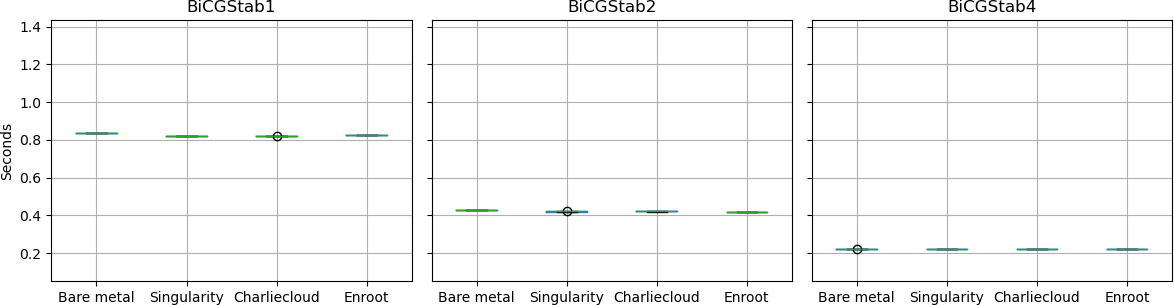
\includegraphics[width=\textwidth]{images/2.png}
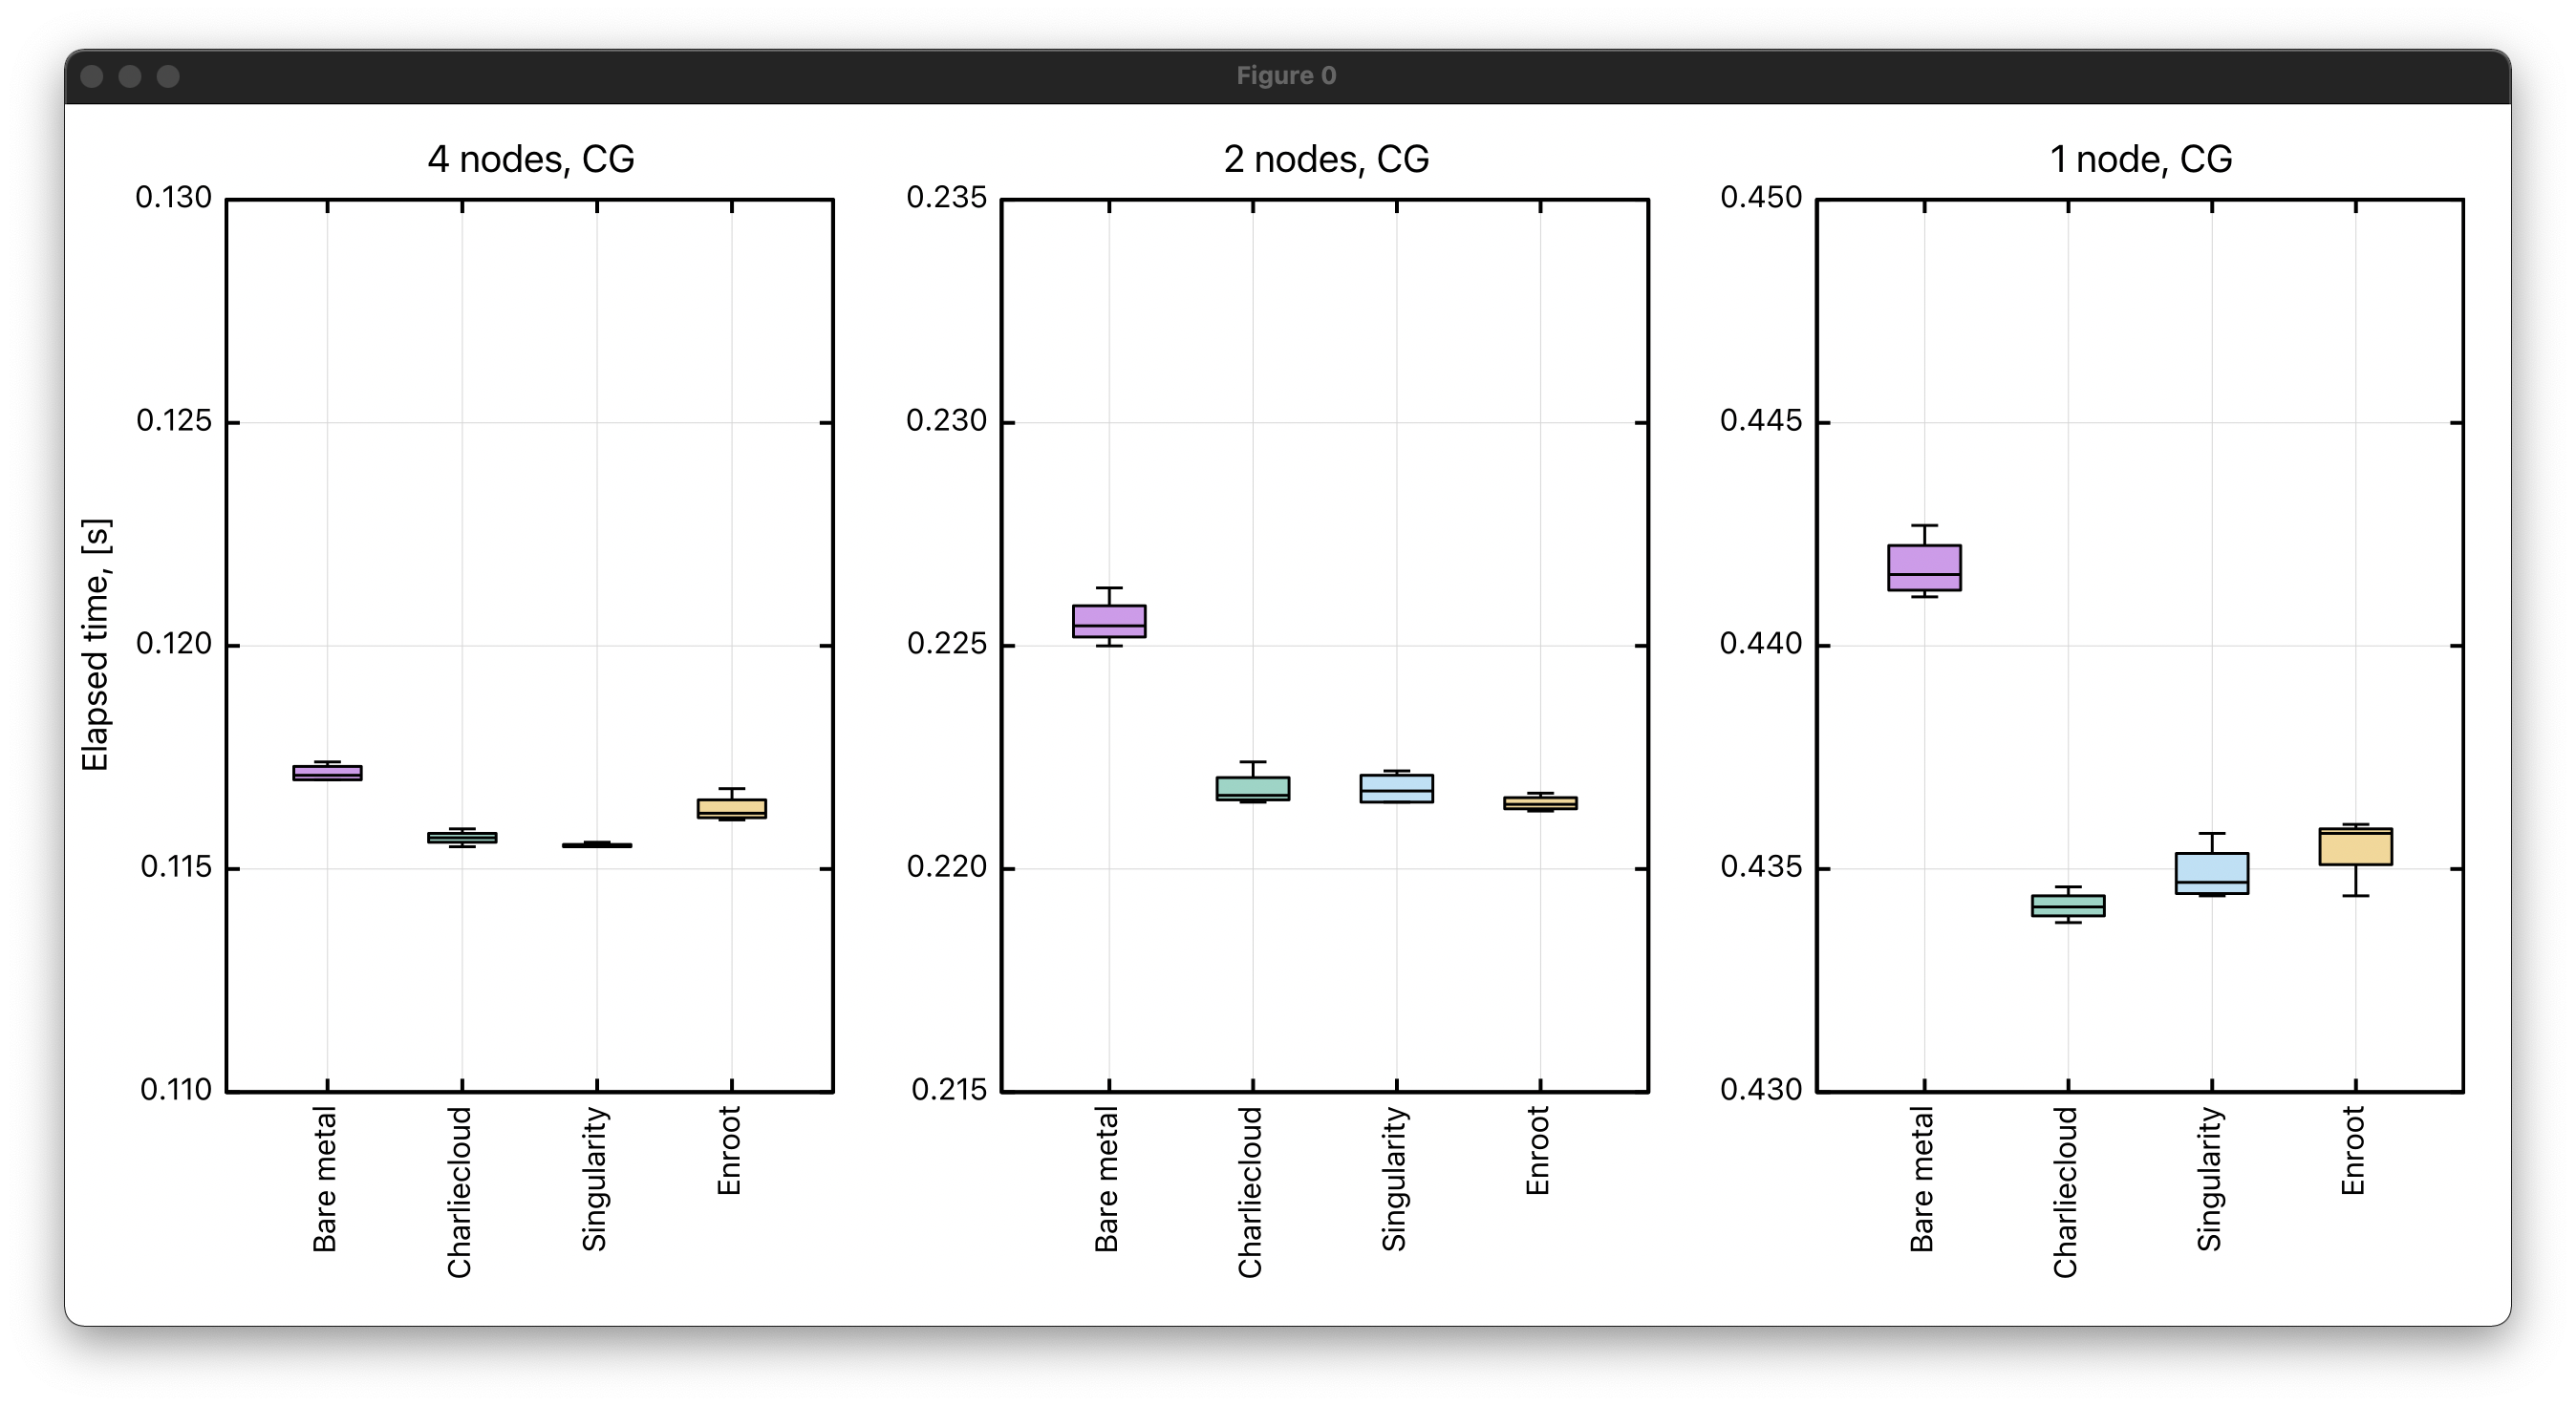
\includegraphics[trim = 40 60 40 60, clip, scale = 0.3]{images/cg.png}
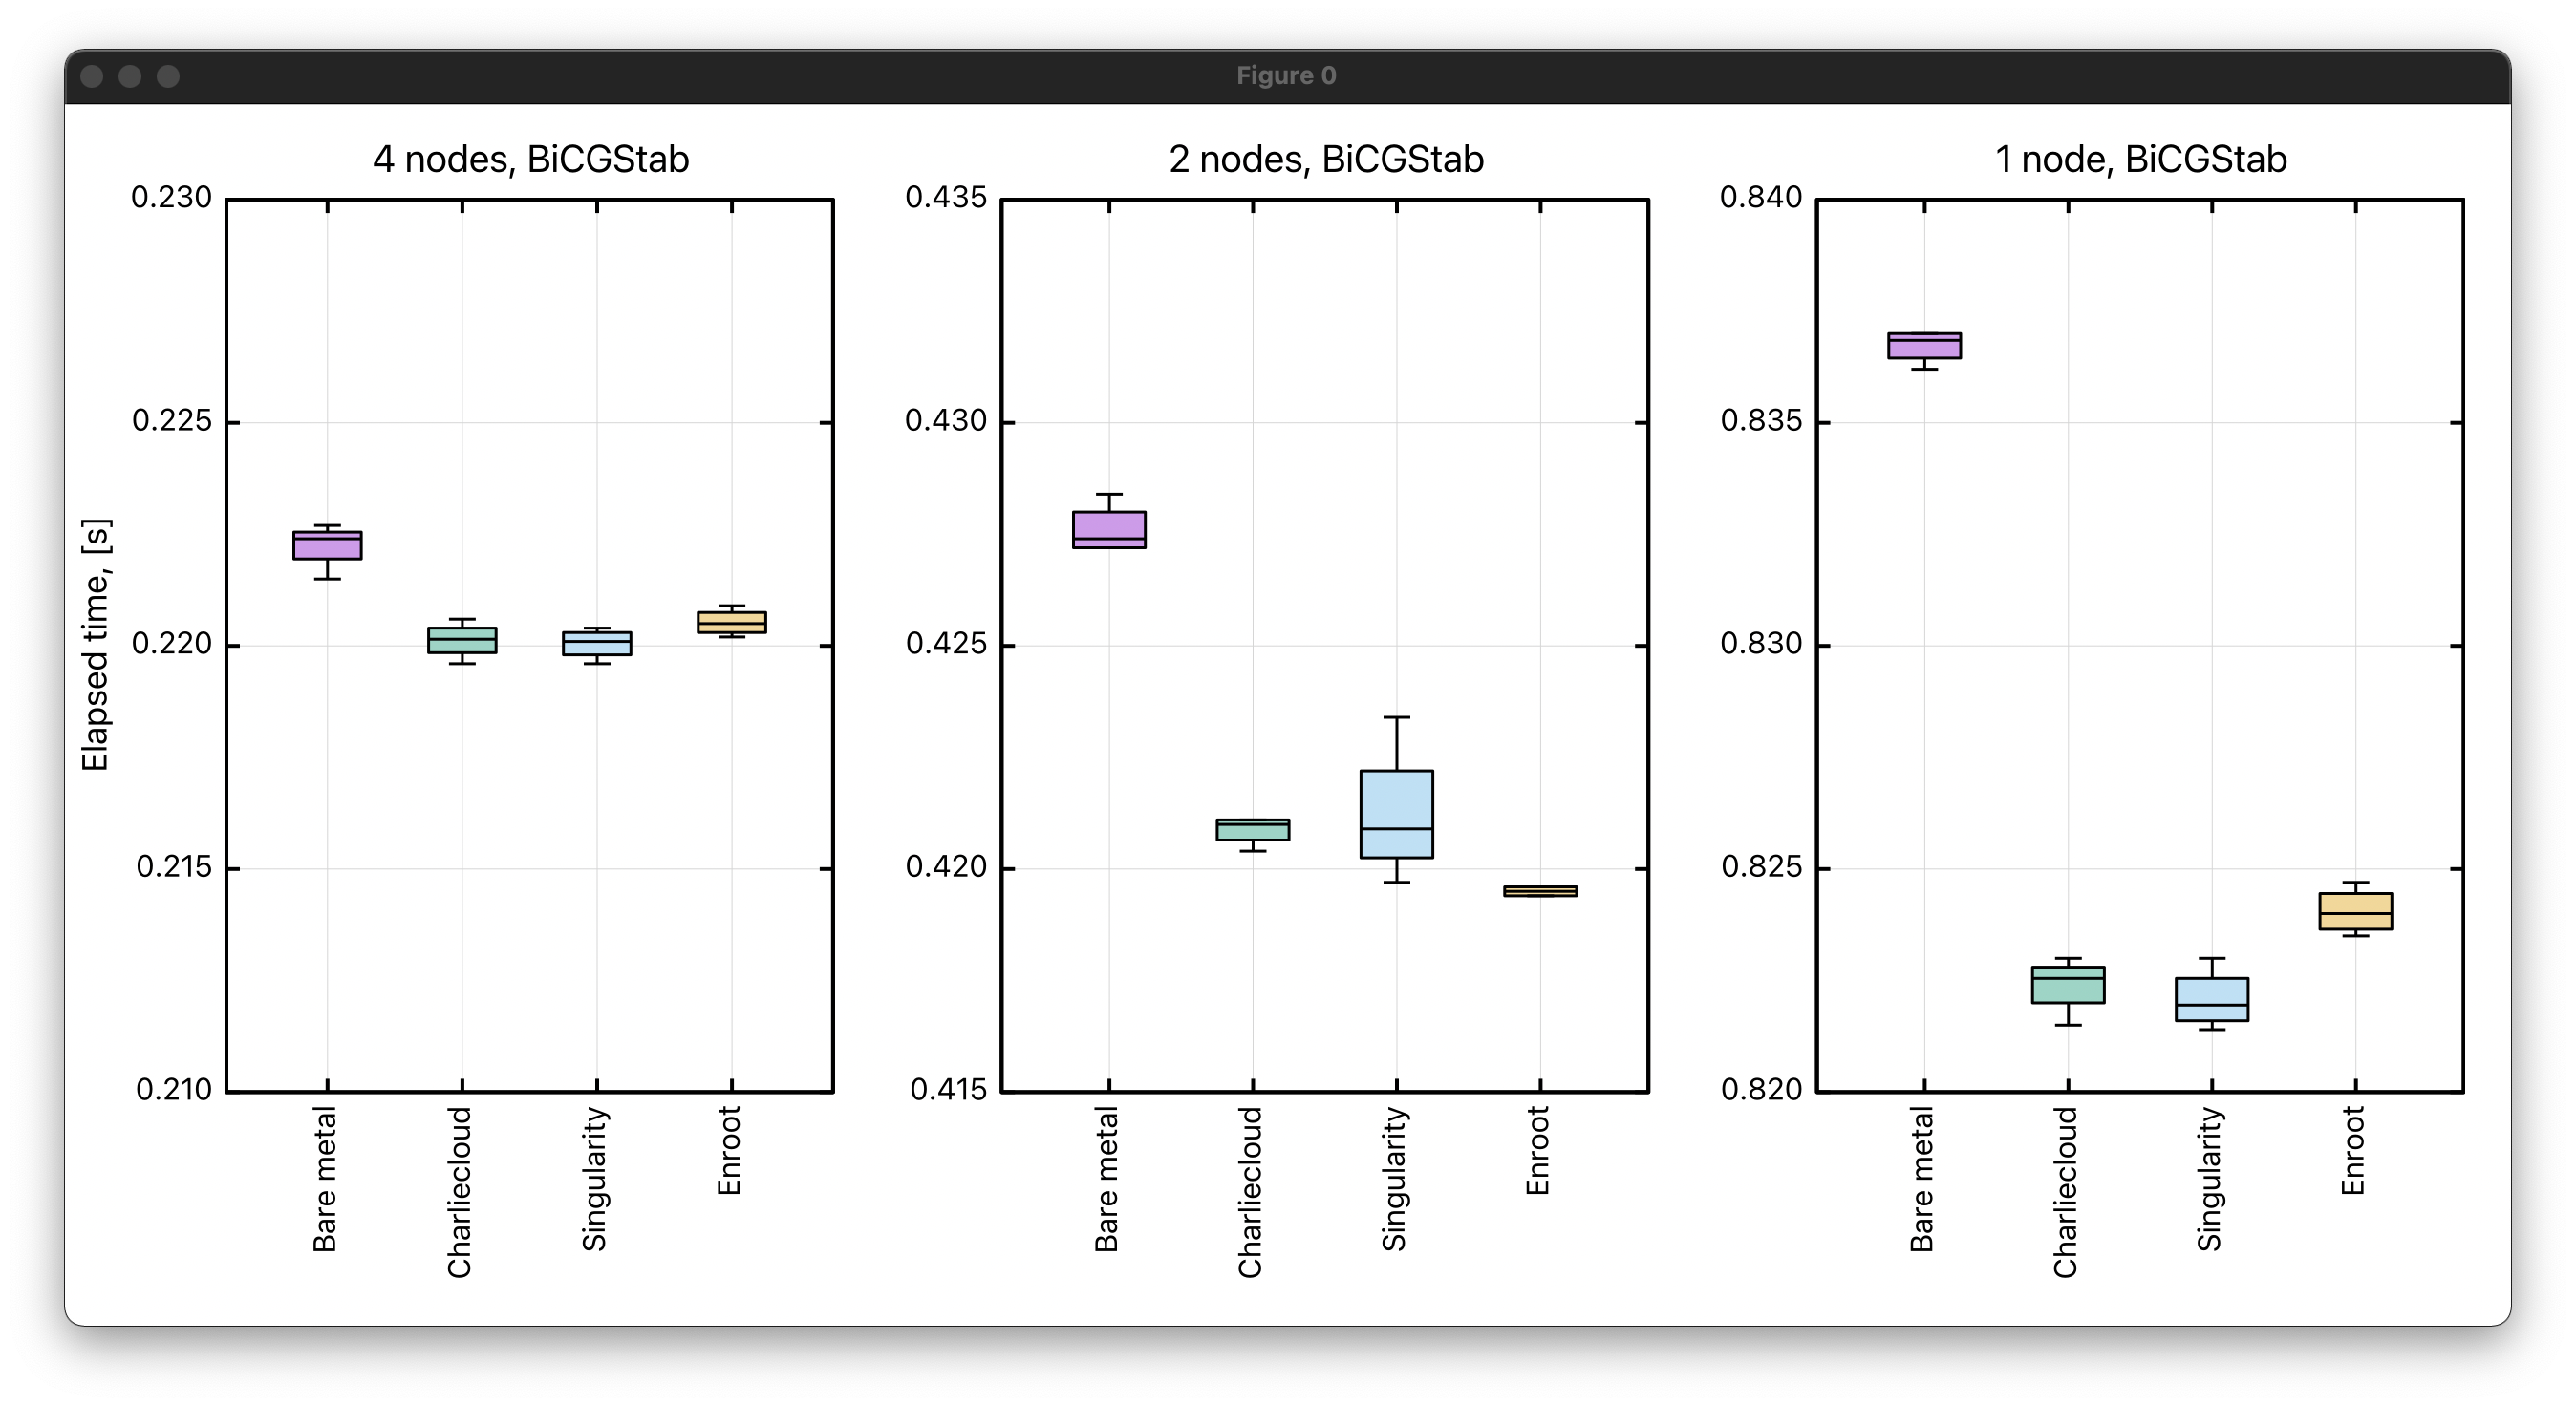
\includegraphics[trim = 40 60 40 60, clip, scale = 0.3]{images/bicgstab.png}
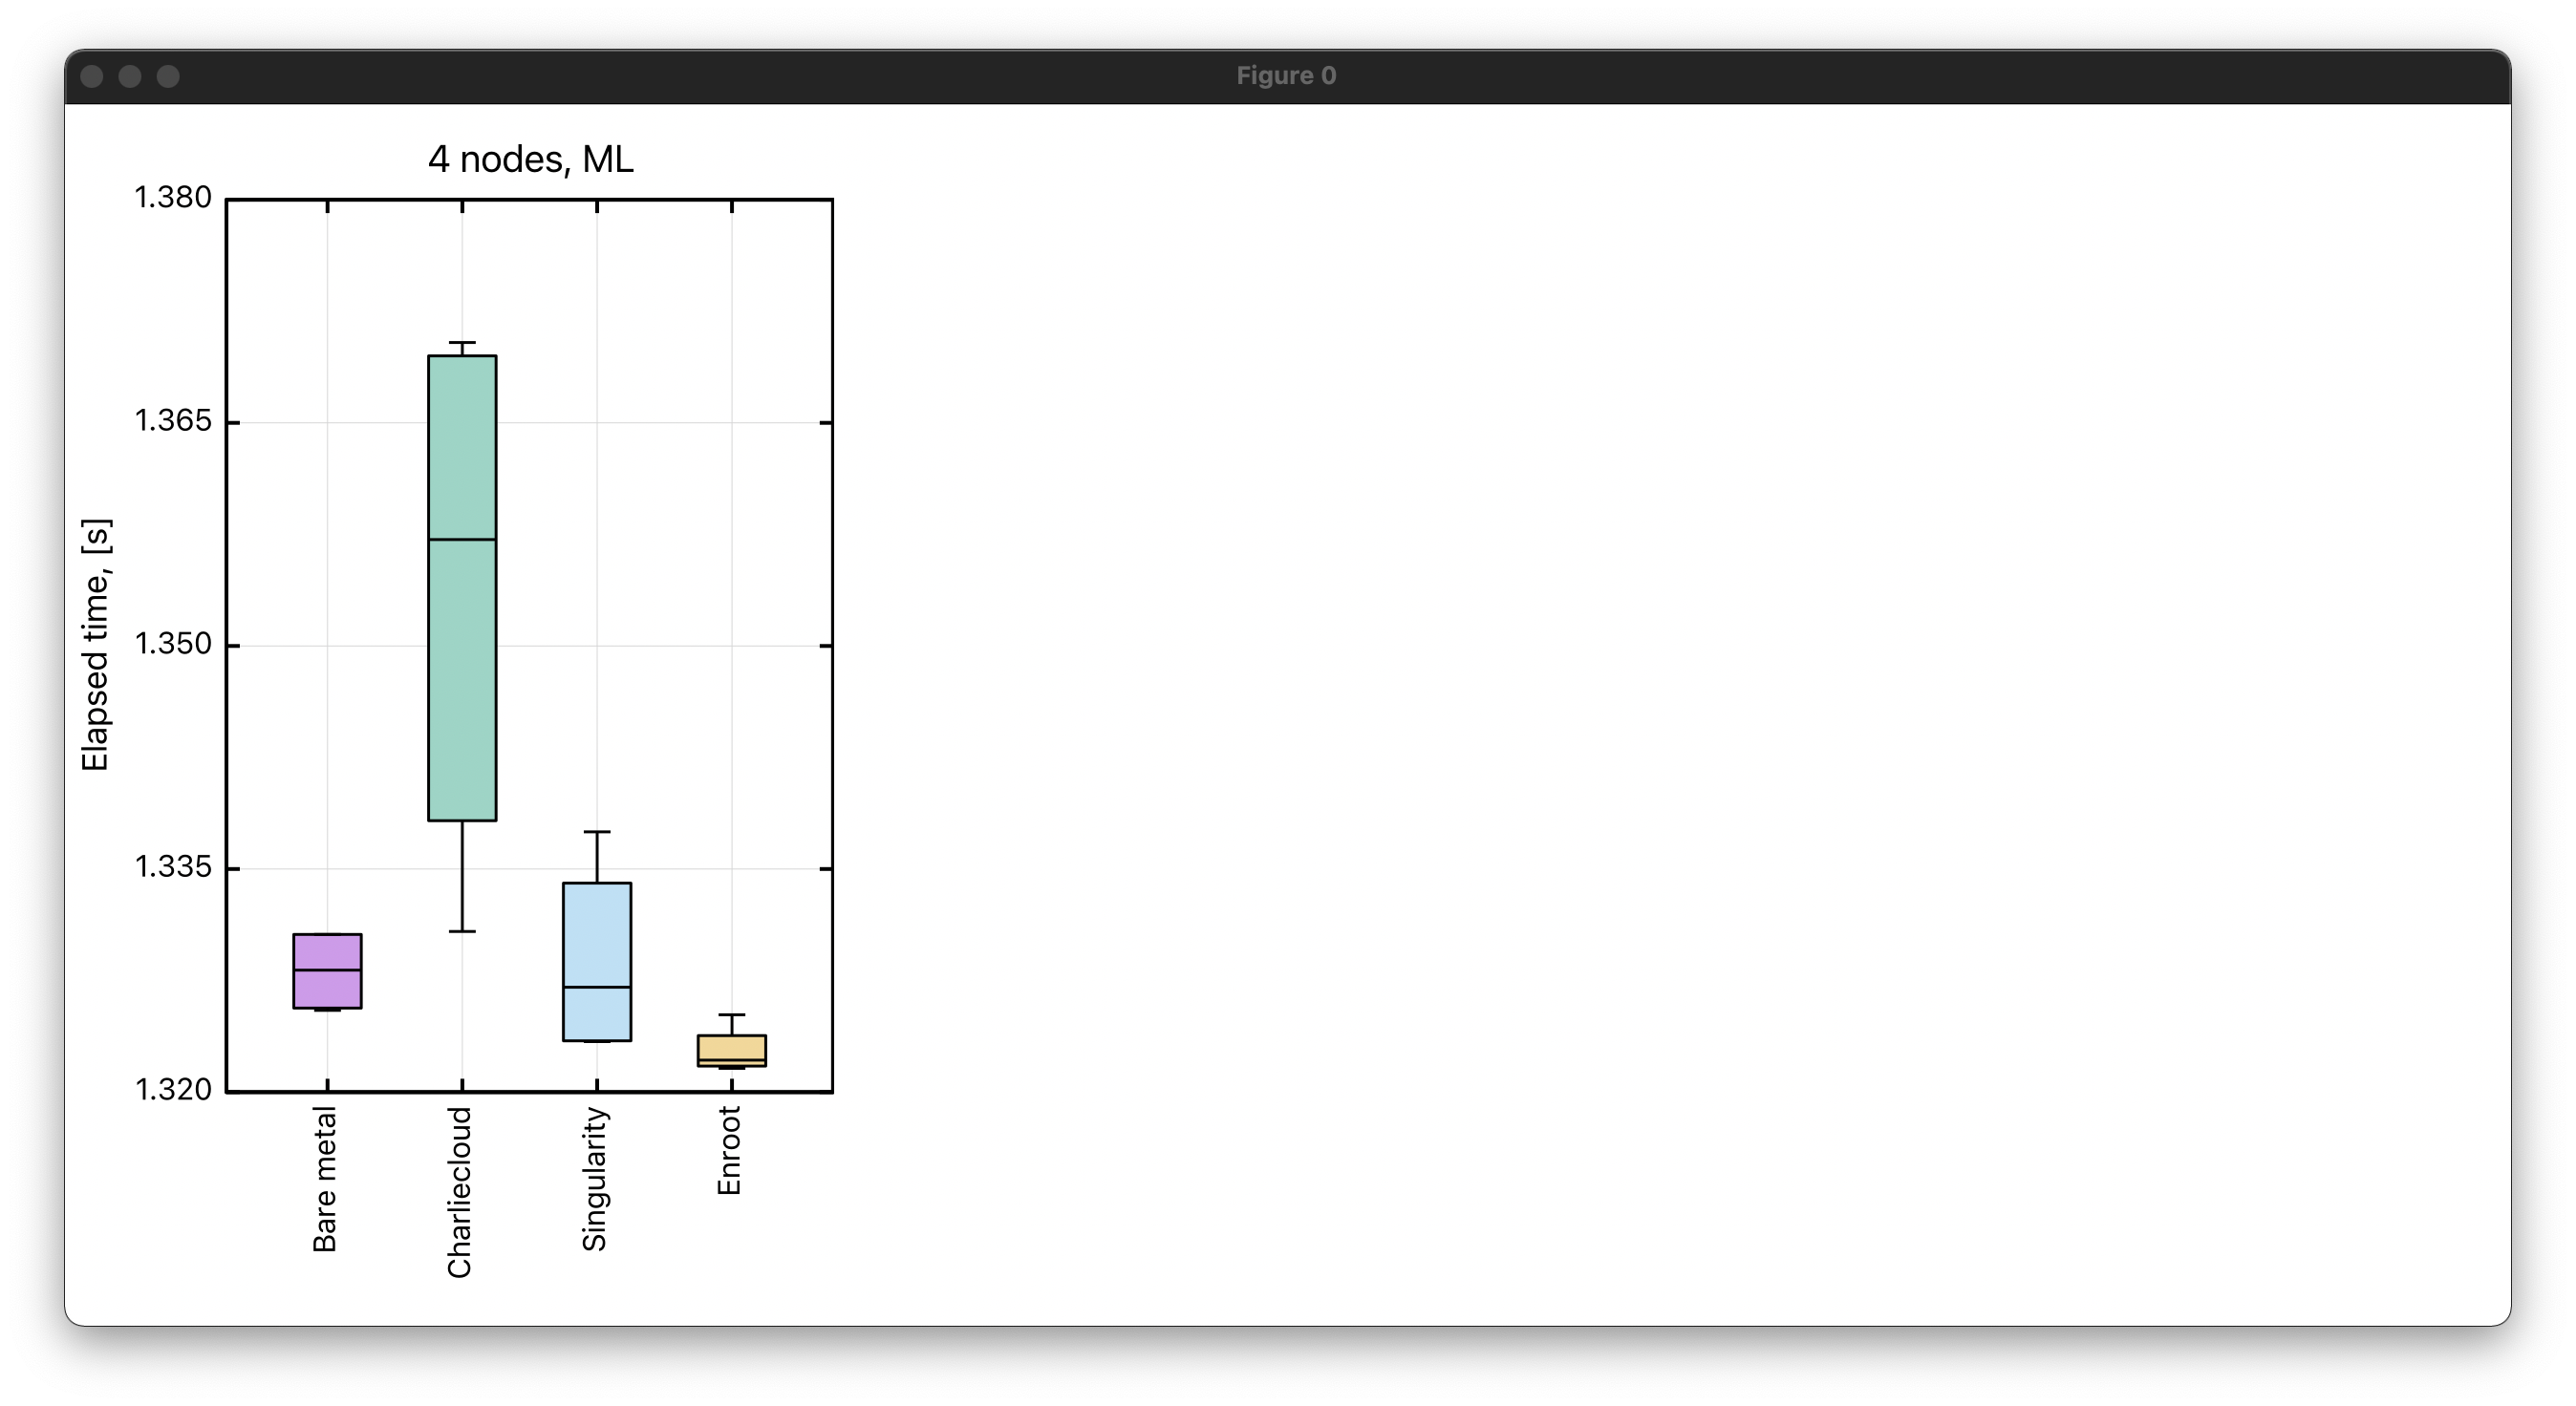
\includegraphics[trim = 40 60 40 60, clip, scale = 0.3]{images/ml.png}
\caption{Comparison of the elapsed time of different linear solvers between different container technologies and bare metal. The benchmarks were executed on four (left), two (middle) and one (right) nodes with 24 cores per node.}
\label{fig:container_benchmarks}
\end{figure}


% \begin{figure}[H]
% \centering
% % 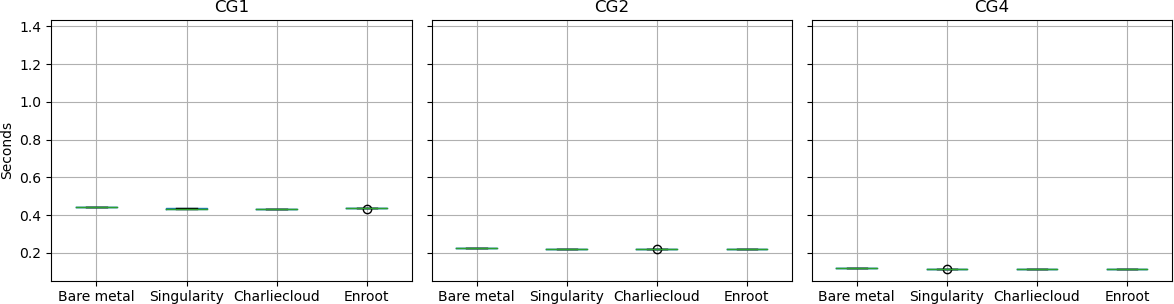
\includegraphics[width=\textwidth]{images/3.png}
% 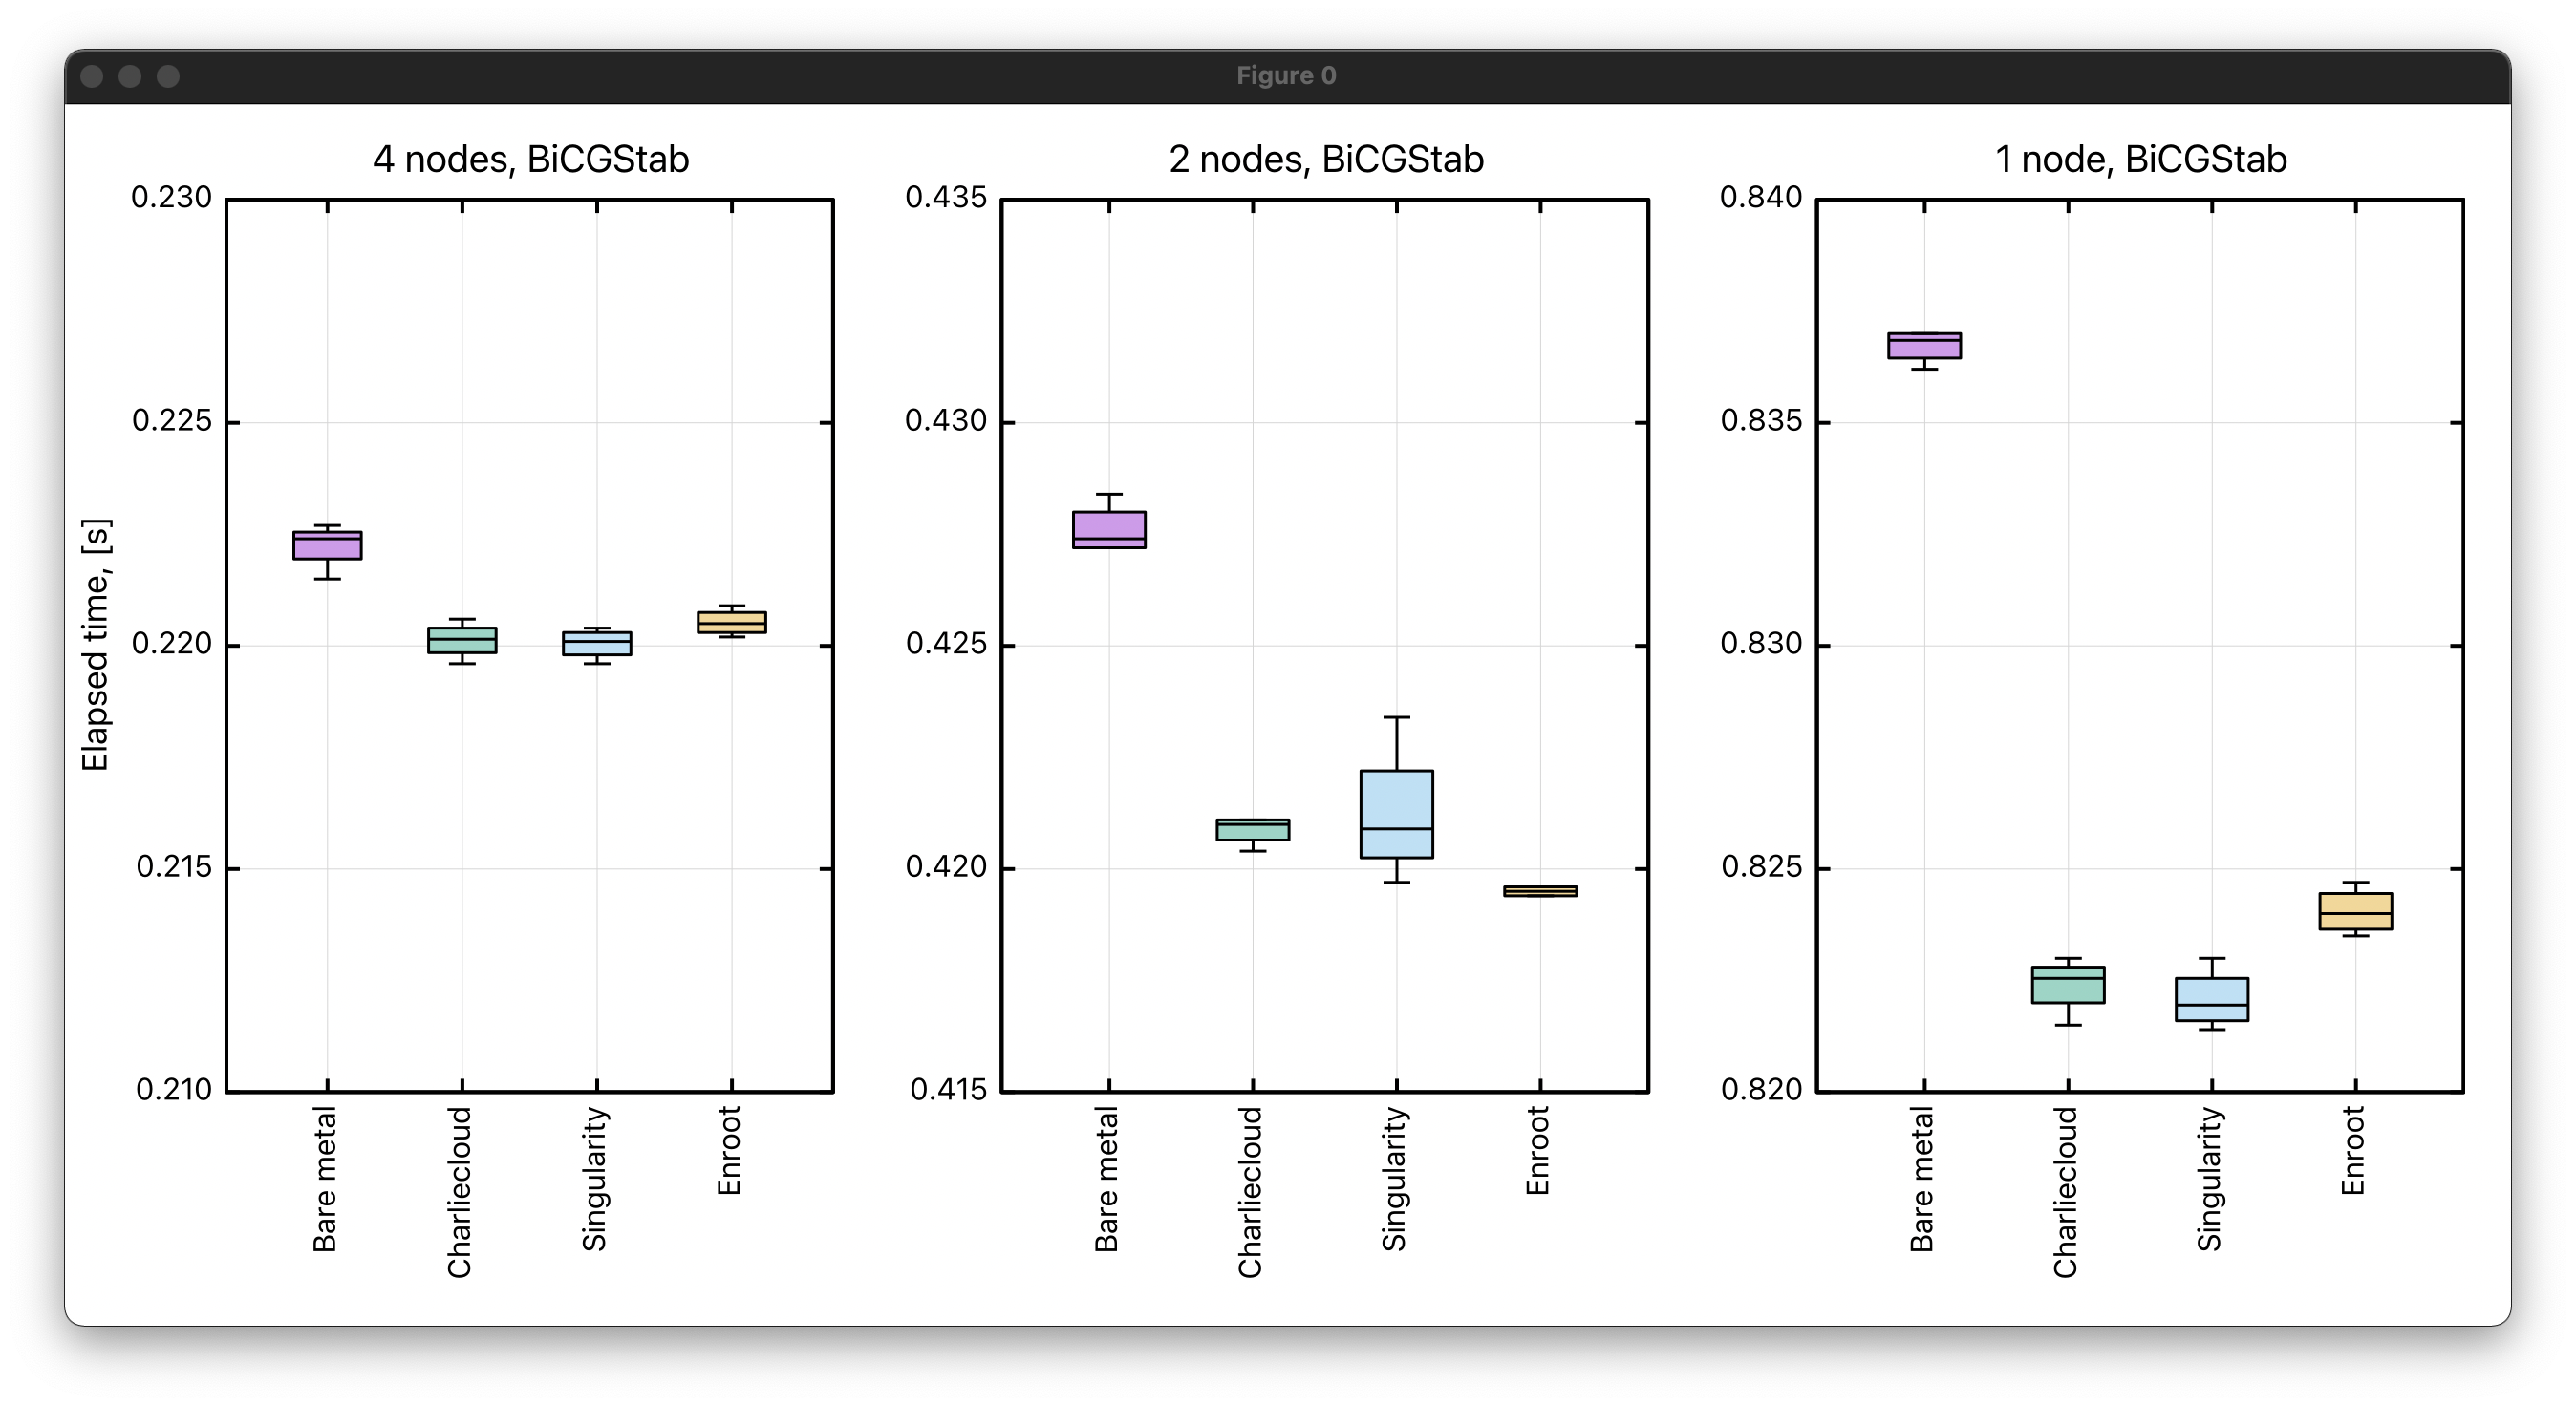
\includegraphics[trim = 40 60 40 60, clip, scale = 0.4]{images/bicgstab.png}
% \caption{Comparison of the elapsed time of the linear solvers between different container technologies and bare metal. Left plots: execution on one node. Middle plots: execution on two nodes. Right plots: execution on four plots.}
% \label{fig:container_benchmarks}
% \end{figure}

% \begin{figure}[H]
% \centering
% % 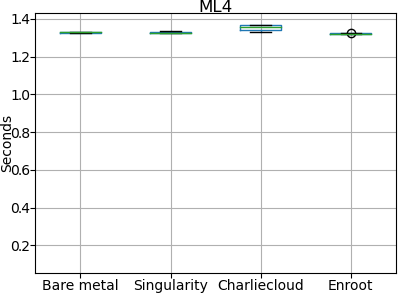
\includegraphics[width=\textwidth/3]{images/1.png}
% 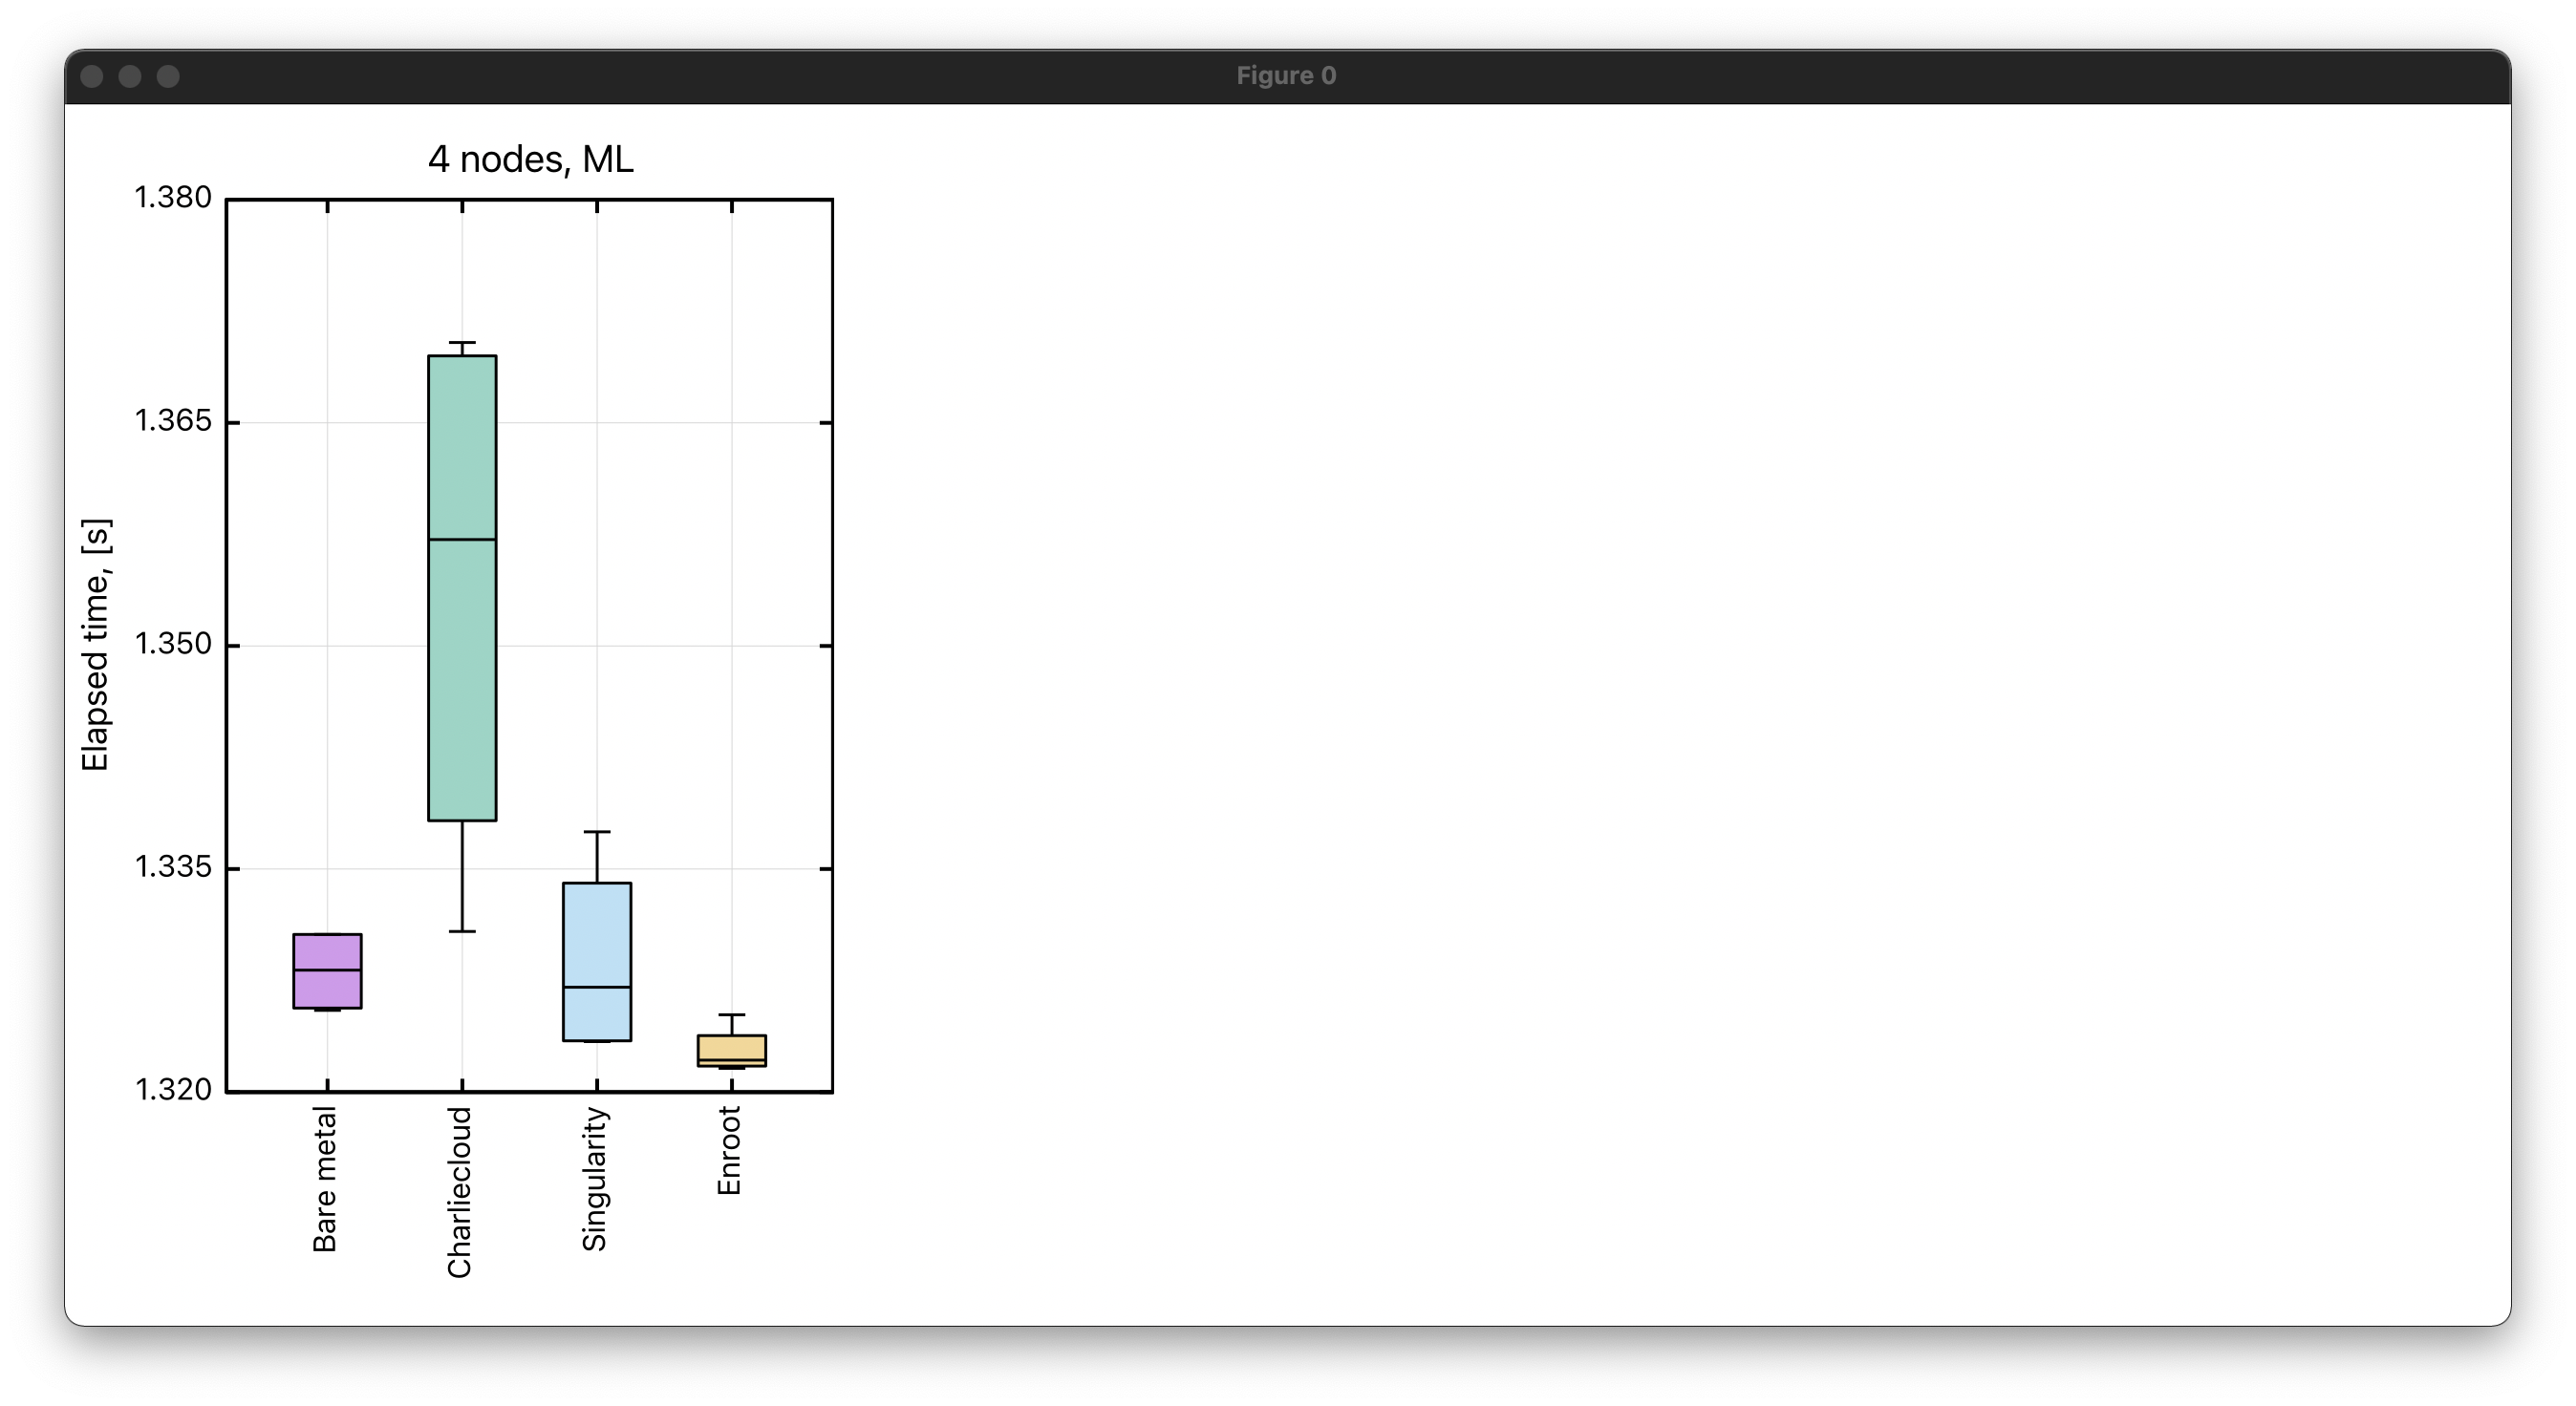
\includegraphics[trim = 40 60 40 60, clip, scale = 0.4]{images/ml.png}
% \caption{Comparison of the elapsed time of the linear solvers between different container technologies and bare metal. Left plots: execution on one node. Middle plots: execution on two nodes. Right plots: execution on four plots.}
% \label{fig:container_benchmarks}
% \end{figure}


\subsection{Container technology in HPC}
    Figure \ref{fig:container_tech} shows the strengths and weaknesses of the evaluated container technologies. The figure is based on an evaluation of nVidia \cite{nvidia-slurm-containers} and represents the most important aspects of the container technologies on a scale from 0 to 5, where 0 is defined as bad and 5 as good. Based on our findings in section \ref{introduction}, we concluded the same results as nVidia for the following subjects: ``Low overhead'', ``Weak isolation'', ``GPU support'', and ``Security''. Furthermore, ``Rootlessness'' is fully based on our evaluation in section \ref{introduction}. The remaining evaluations are based on section \ref{introduction} and our experiences with the container technologies on our \gls{hpc} system.
    
 % -----------------------------------------------------------
    
%     singularity more mature (better documentation)
    
%     singularity is more complex to use than other tools (needs examples, since better documentation makes this a strange conclusion) - many more commandline options. enroot most of the time has intermediate steps, it's more basic, but has this as a tradeoff.
    
%     enroot takes more time to setup due to the pyxis plugin, however, this plugin allows better fine grained multi-node support compared to the other solutions? this was harder with the other tools? the other containers were executable as a file via srun, right? maybe needs this detailed a bit more explained
    
%     rootless section is in more detail explained in the introduction section about these tools. such as explained: they all use namespace separation (suduid) and enroot may build containers as normal user by the use of buildah. so for building mpi inside an enroot container, buildah would've been your friend :)
%     adding the CVE about security issues is a good one, will add that in the introduction section.
    
%     using user namespaces makes transparent filesystems such as network filessytems (lustre/nfs) unsuable for fakeroot containers because the filesystem is not aware of this uid/gid mapping. good that you mentioned this, i'll add it
    
%     > Only Enroot has direct integration with SLURM via the Pyxis plugin
%     all the containers were executable files, right? these can be used in an srun or sbatch, correct? in what way did pyxis provide more features/support with slurm?
    
%     > Singularity and Charliecloud allow using of archived images
%     with this you mean something like dockerhub? or importing pre-build containers from a shared filesystem/repository? - archive is tarball (e.g. sif). enroot cannot convert tarball to squasfs, less universal
    
%     i have no comments about the cross-platform part, looks good :)
    
    
%                             singularity - charliecloud - enroot
% low overhead            3 (5)           5             5
% weak isolation          2               5             5
% GPU                     2 (4)           2             5
% mpi support             3 (4)           3 (4)         4 (3)
% slurm integration       3 (0)           3 (0)         4 (5)
% security                3               4             4      
    
% ---------------------------------------------------------------
    
    \begin{figure}[H]
    \centering
    % 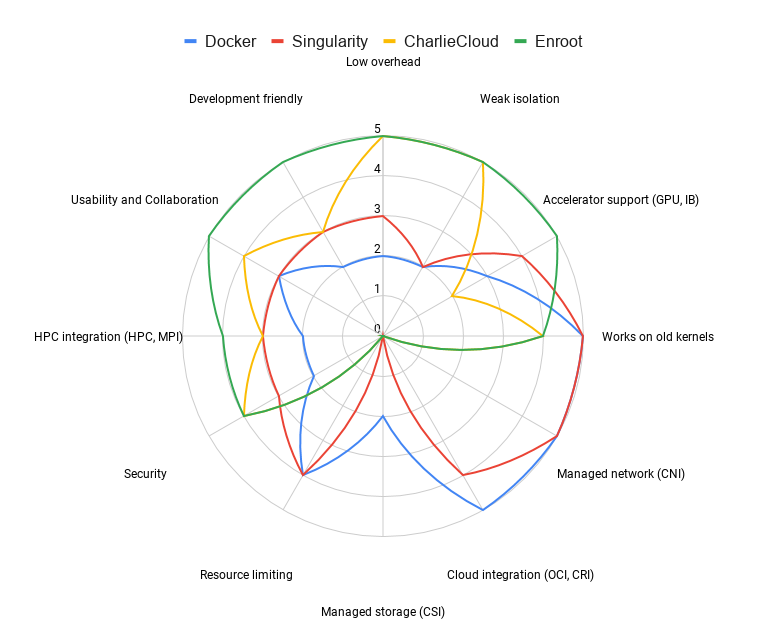
\includegraphics[width=400px]{images/container_tech.png}
    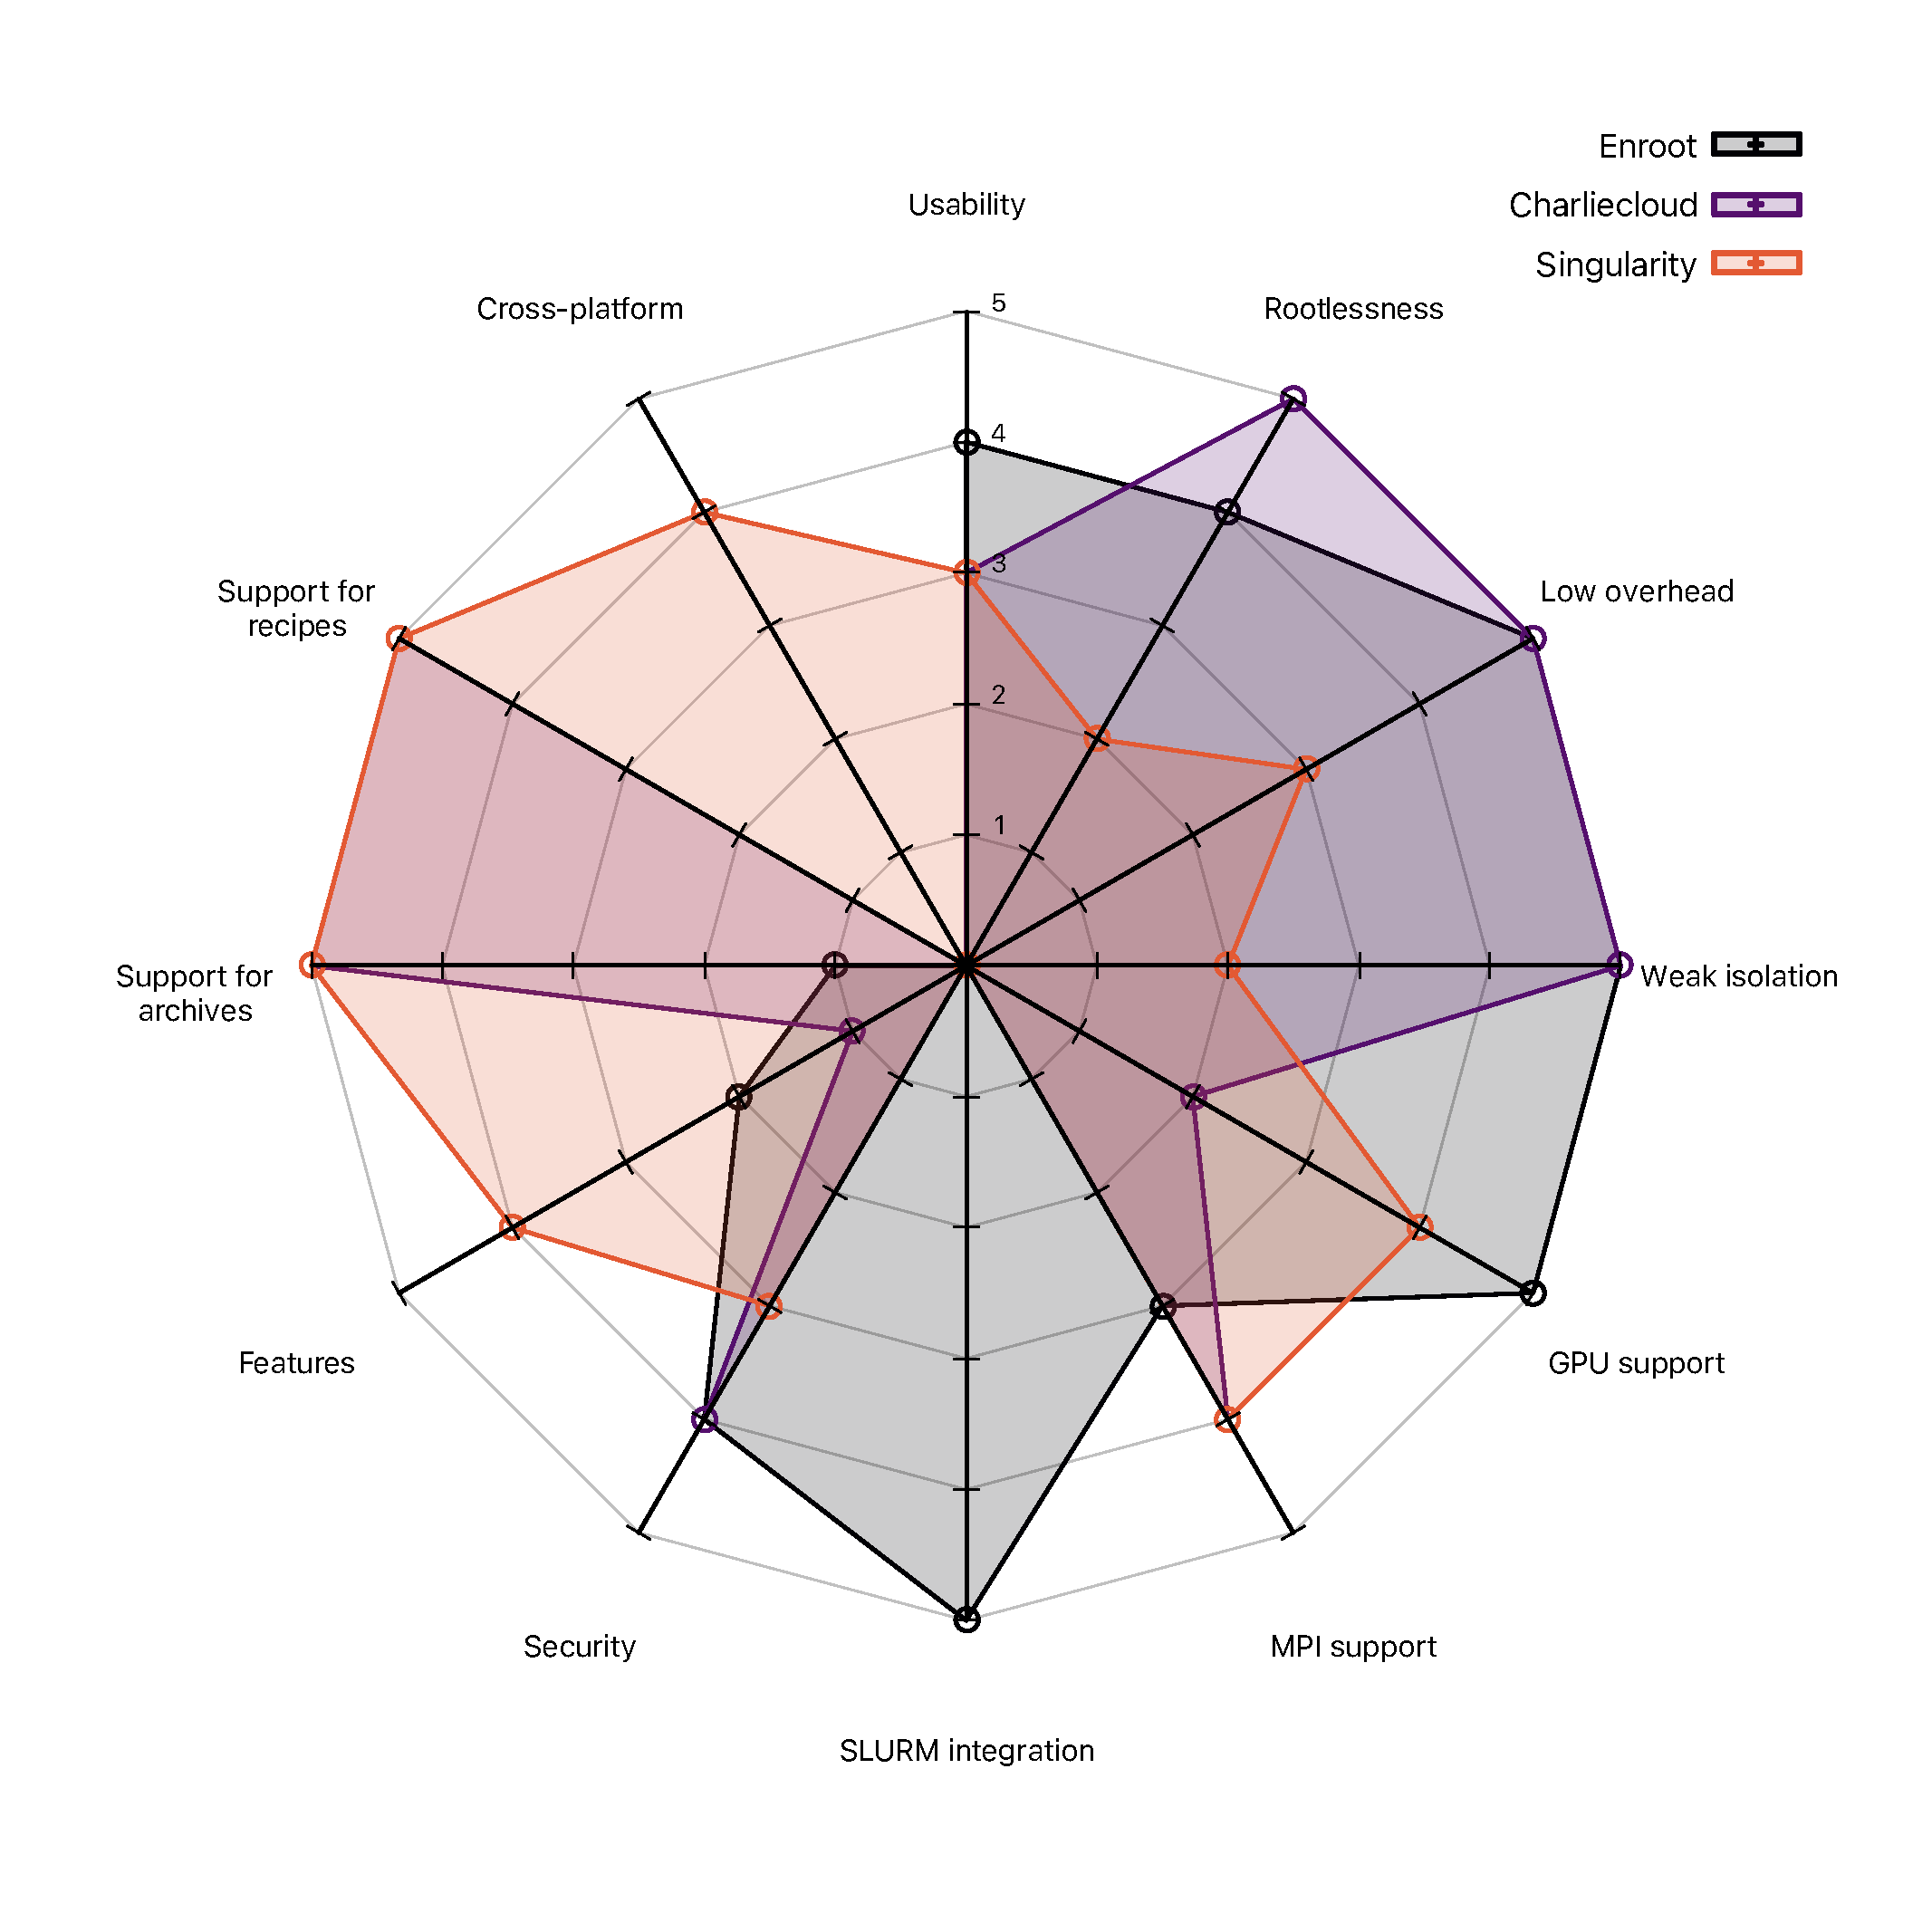
\includegraphics[scale=0.35]{images/containers_spider.pdf}
    \caption{Strenghts and weaknesses of the tested container technologies.}
    \label{fig:container_tech}
    \end{figure}

    \subsubsection{Usability, features, and support for archived images}
    In terms of usability from the users' perspective; Singularity has 78 manuals stored in \linebreak \mintinline{bash}{/usr/share/man/}, which reflects the amount of command line arguments available. This benefits Singularity in terms of features. However, it also makes it slightly harder to find the required information when a user does not know where to look. In comparison, Charliecloud is packaged with 20 manuals. Enroot went even further, by not including any manuals.
    
    However, the online documentation of enroot was sufficient. Enroot's features are more basic and thus getting to know the tool and finding out all the features was easier. We noticed one missing feature, i.e. the ability to create archived images (tarballs). This feature simplifies the utilization and execution of the containers that can be built off-site.
    
    The usability in terms of the engineers' perspective was not taken into account in this evaluation. However, we would like to note that Singularity and Charliecloud had the best support for \gls{rhel} systems. We had to build and maintain our own RPMs for enroot\footnote{\url{https://fedorapeople.org/cgit/keesdejong/public_git/rpmbuild.git/tree/SPECS/enroot.spec}} \footnote{\url{https://fedorapeople.org/cgit/keesdejong/public_git/rpmbuild.git/tree/SPECS/pyxis.spec}}.
    
    \subsubsection{SLURM and MPI support}
    In terms of \gls{hpc} integration, i.e. \gls{mpi} and \gls{slurm} support, enroot performed better by providing a \gls{slurm} plugin. The enroot Pyxis plugin significantly simplifies the utilization of the container technology on an HPC system. This, for instance, allows users to rely on system-defined rules for core affinity and core binding. Furthermore, all tested containers allow to compile and execute MPI applications in the container. However, enroot does not provide their own solution to build containers. Buildah (from Red Hat) is used to build a container without privileges. The built container then has to be converted to the enroot format.
    


    % \subsubsection{Usage complexity}
    % \textit{Determines how hard it is to use container technology from the user's perspective.} Singularity can be considered as the most mature technology among all tested containers. Singularity has good documentation and is already used on many HPC systems. However, Singularity is also the most complex technology tested. Thus, Singularity has a steeper learning curve compared to Charliecloud and Enroot.

    % \subsubsection{Set up complexity}
    % \textit{Determines how hard is container technology to set up on the HPC system.} We found that Enroot takes more time to set up. This is because Enroot requires the installation of the Pyxis, a SPANK plugin for the SLURM workload manager, in order to allow execution of multi-node tasks. [something else? something about lustre and nfs? Kees: nothing else, the filesystem issues were on all container technologies because they don't support namespaces. there was no huge difference in mpi support? or to get things working? otherwise this is fine]
    
    % \subsubsection{Rootlessness} 
    % \textit{Determines if a container can be built and run by an unprivileged user.} All three solutions can be used to run containers by unprivileged users. However, only Charliecloud allows building containers in a fully unprivileged mode. Singularity supports the usage of a "fakeroot" option. However, to allow users to build containers from the recipe files, Singularity requires users to be added to the SUBUID list. This may compromise the security of the system and, therefore, expose the system to potential attacks \textbf{[can it?, yes it can, i can add some CVEs, but they all use the subuid/subgid mappings, also charliecloud: https://hpc.github.io/charliecloud/command-usage.html]}. To build containers with Enroot one should either have access to registries (e.g. Docker Hub), or to the Docker daemon running on the same system as Enroot. Due to security concerns, the Docker daemon cannot be executed on public HPC systems. However, Enroot can make use of the Red Hat tool Buildah, which allows to build containers without root privileges by the use of namespace separation.

    % \subsubsection{GPU support}
    % Determines is technology suppors GPU accelerators. According to the official documentation [ref.], only Enroot has direct support for GPU accelerators. Other containers may work with GPUs, but the setup might be tedious. We didn't perform tests with GPU accelerators and, therefore, rely on open resources to evaluate this field.
    
    % \subsubsection{MPI support}
    % \textit{Determines how easy it is to install MPI libraries and use HPC codes.} All tested containers allow to compile and execute MPI applications in the container. However, our tests showed that the installation of MPI inside the container, against existing SLURM installation on the host, are much easier with Singularity and Charliecloud compared to Enroot. This is because Enroot can't build directly from the recipe files. This constraint significantly complicates the installation of the MPI library, which requires the execution of the following steps:
    % \begin{itemize}
    %     \item Creating the basic (only OS and the most necessary packages) docker image on the local machine.
    %     \item Uploading the created docker image to the registry.
    %     \item Downloading the image from the registry to the HPC machine and creation of the squashfs image.
    %     \item Unsquashing the image.
    %     \item Adding changes to the unsquashed image (installing MPI, adding symbolic links to SLURM from the host system, etc.).
    %     \item Squashing the image back.
    % \end{itemize}
    
    % \subsubsection{SLURM integration}
    % \textit{Determines if technology has integration with SLURM.}
    % Only Enroot has direct integration with SLURM via the Pyxis plugin. The Pyxis plugin significantly simplifies the utilization of the container technology on an HPC system. This, for instance, allows users to rely on system-defined rules for core affinity and core binding.
    
    % \subsubsection{Features}
    % Among all, Singularity is the most advanced and the most mature technology. [why? what does it have?]
    
    % \subsubsection{Support for archives} 
    % \textit{Determines if the technology can use archived images.} Singularity and Charliecloud allow using of archived images that were built and transferred from the remote machine. This significantly simplifies the utilization and execution of the containers that can be built off-site. In contrast, Enroot does not provide this feature.
    
    \subsubsection{Support for recipes}
    Singularity and Charliecloud support the utilization of the recipe files to specify a container build. Charliecloud allows the use of the industry-standard ``Dockerfile'', whereas Singularity can operate only with recipe files of its own format. Enroot can only operate with images from registries and can only use a limited functionality of so-called configuration files.
    
    \subsubsection{Cross-platform}
    Only Singularity can be considered as a cross-platform container solution (with some limitations and complexities on Mac machines). The two other container technologies can be run only on Linux-based systems.


\subsection{Container orchestrators in HPC}
\label{containers_hpc}
In this section we will discuss the strengths and weakness of \gls{slurm} and Kubernetes in \gls{hpc}.

\subsubsection{Performance}
Futral researched the performance differences of several batch schedulers, including \gls{slurm} and Kubernetes \cite{futral2019method}. The researcher's measurements were wall clock time, RAM usage, and CPU usage. These measurements captured the utilization of system resources for each of the schedulers. The batch jobs were composed of custom scripts, using the NASA Parallel Benchmark programs and computational fluid dynamics, which were executed using, 1, 2, and 4 servers to determine how well a scheduler scales with network growth. All hardware was similar and was co-located within the same data-center.

Kubernetes performed less than \gls{slurm}. For instance, Kubernetes needed to determine if Weave-Net was the appropriate network plugin for the cluster before starting a container. This overhead resulted in a slower time-to-spool. Furthermore, Kubernetes did not perform well because the worker pods had to be first provisioned before a controller pod could be provisioned via the batch job. Kubernetes also consumed the most RAM. Furthermore, the Kubernetes cluster also suffered from utilizing SSH for its communication protocol. This was due to the extra overhead of encryption in SSH. \gls{slurm} does not use encryption, \gls{slurm} only authenticates communication with a distributed symmetric key (MUNGE). In addition to SSH, the Kubernetes setup also relied on a virtual network and custom dynamic DNS solutions to determine worker node availability. The added layer of the virtual network and the DNS lookups significantly affected Kubernetes' its performance. In \cite{futral2019method}, \gls{slurm} performed best and did not appear to require any optimizations in terms of additional configuration of the supporting OpenMPI libraries themselves.

While Kubernetes does provide some batch job facilities, ease of development, and process isolation; the research concluded that it overall did not perform as well as expected. In conclusion, the data that was collected suggests that most batch schedulers are uniquely tuned to improve performance of high-performance compute jobs. This advanced tuning was especially pronounced in \gls{slurm}, and less pronounced with Kubernetes.

\subsubsection{HPC workloads}
``Embarrassingly parallel'', or ``perfectly parallel'' applications on a Kubernetes cluster can launch multiple containers in parallel, but the scale is ``best effort'' at launch time as ``gang scheduling'' is not possible; also it is not possible for the application to perform different functions on the ``primary'' container as the ``secondaries'', so sharding and setup must be performed either in advance or manually. This is not architecturally compatible with most existing applications \cite{hpc-on-kubernetes}. This makes a Kubernetes cluster not suitable as a tightly-coupled parallel solver as it cannot guarantee scale neither at launch nor at runtime.

Accelerated parallel training for AI on Kubernetes is not supported for the same reasons as for parallel solvers; alternative training workflows must be used (assuming framework support) when scale is needed. However, AI workloads for accelerated real-time analytics is supported. Assuming Kubernetes plugins exist for accelerated hardware, it may support these stacks.

Many \gls{hpc} applications have specific requirements relative to where they are executed within the system. Where each task (rank) of an application may need to communicate with specific neighboring tasks and so prefer to be placed topologically close to these neighbors to improve communication with these neighbors. This is called topology-aware scheduling. Other tasks within the application may be sensitive to the performance of the I/O subsystem and as such may prefer to be placed in areas of the system where I/O throughput or response times are more favorable \cite{stackhpc-kubernetes-mpi}. As of writing this report, Kubernetes may only make this possible by manual scheduling containers on specific hosts in the cluster. In \gls{slurm} however, this is a builtin feature.

\subsubsection{MPI support}
\gls{slurm} also has builtin support for \gls{mpi} such as Intel-MPI, MPICH2, MVAPICH2, OpenMPI, PMIx and UPC. \gls{mpi} use depends upon the type of \gls{mpi} being used. There are three fundamentally different modes of operation used by these various \gls{mpi} implementation. 1) \gls{slurm} directly launches the tasks and performs initialization of communications through the PMI2 or PMIx APIs. 2) \gls{slurm} creates a resource allocation for the job and then mpirun launches tasks using \gls{slurm}s infrastructure. And 3) \gls{slurm} creates a resource allocation for the job and then mpirun launches tasks using some mechanism other than \gls{slurm}, such as SSH or RSH. These tasks are then initiated outside of \gls{slurm}s monitoring or control \cite{slurm-pmi}.

There are projects underway with the goal of integrating Kubernetes with \gls{mpi}. One notable approach, kube-openmpi, uses Kubernetes to launch a cluster of containers capable of supporting the target application set. Once this Kubernetes namespace is created, it is possible to use kubectl to launch and mpiexec applications into the namespace and leverage the deployed OpenMPI environment. kube-openmpi only supports OpenMPI, as the name suggests.

Another framework, Kubeflow, also supports execution of MPI tasks atop Kubernetes. Kubeflow’s focus is evidence that the driving force for MPI-Kubernetes integration will be large-scale Machine Learning. Kubeflow uses a secondary scheduler within Kubernetes, named kube-batch, to support the scheduling and uses OpenMPI and a companion SSH daemon for the launch of \gls{mpi}-based jobs. Such approaches do not fully leverage the flexibility of the elastic Kubernetes infrastructure, or support the critical requirements of large-scale \gls{hpc} environments.

In some respects, kube-openmpi is another example of the fixed use approach to the use of containers within \gls{hpc} environments. For the most part there have been two primary approaches. Either launch containers into a conventional \gls{hpc} environment using existing application launchers (e.g., Shifter, Singularity, etc.), or emulate a conventional data parallel \gls{hpc} environment atop a container deployment orchestrator with kube-openmpi.

\subsubsection{Resource management}
Kubernetes 1.18 enables a new feature called Topology Manager \cite{gridengine-topology}. This is a component of kubelet which also takes care of NUMA optimizations, which runs locally on the target host. Topology Manager provides host local logic, which enables; 1) only host local decisions and 2) lead to wasted resources when pods needs to be re-scheduled many times to find a host which fits. The Topology Manager provides following allocation policies: none, best-effort, restricted, and single-numa-node. These are kubelet flags. The actual policy which is applied to the pod depends on the kubelet flag but also on the QoS class of the pod itself. The QoS class of the pod depends on the resource setting of the pod description. If CPU and memory are requested in the same way within the limits and requests section then the QoS class is guaranteed. Other QoS classes are best-effort and burstable. The kubelet calls so called Hint Providers for each container of the pod and then aligns them with the selected policy, like checking if it works well with the single-numa-node policy. When set to restricted or single-numa-node it may terminate the pod when no placement is found so that the pod can be handled by external means (like rescheduling the pod). Some interesting development efforts and functionalities already in place for Kubernetes \cite{kubecon-2018}.

\begin{itemize}
    \item CPU Pinning and Isolation
    \item Device Plugins (GPUs, Infiniband, FPGA, etc)
    \item NUMA Management
    \item SR-IOV Networking plugin
    \item Spark 2.3.0 with Kubernetes scheduler instead of Yarn
    \item Pods Priorities and Preemption
    \item Container Runtime
        \begin{itemize}
        \item CRI-O - OCI stable runtime follow rootless
        \item KataContainers - OCI VM Containers
        \item Singularity - Syllabs seems to be working on support of Kubernetes
        \item Gvisor - Google sandboxed containers
    \end{itemize}
    \item Kubernetes cluster federation – for offloading on hybrid clouds
    \item Kubeflow to make machine learning simple, portable and scalable
\end{itemize}

\subsubsection{Infrastructure deployment methods}
The Kubernetes blog provides several suggestions for \gls{hpc} deployments \cite{kubenetes-blog-meets-hpc}. 1) Maintain separate infrastructures. For sites with sunk investments in \gls{hpc}, this may be a preferred approach. Rather than disrupt existing environments, it may be easier to deploy new containerized applications on a separate cluster and leave the \gls{hpc} environment untouched. The challenge is that this comes at the cost of siloed clusters, increasing infrastructure and management cost.

2) For sites running traditional \gls{hpc} workloads, another approach is to use existing job submission mechanisms to launch jobs that in turn instantiate containers on one or more target hosts. Sites using this approach can introduce containerized workloads with minimal disruption to their environment. Leading \gls{hpc} workload managers such as Univa Grid Engine Container Edition and IBM Spectrum LSF are adding native support for containers. Shifter and Singularity are important open source tools supporting this type of deployment also. While this is a good solution for sites with simple requirements that want to stick with their \gls{hpc} scheduler, they will not have access to native Kubernetes features, and this may constrain flexibility in managing long-running services where Kubernetes excels.

3) Use native job scheduling features in Kubernetes. Sites less invested in existing \gls{hpc} applications can use existing scheduling facilities in Kubernetes for jobs that run to completion. While this is an option, it may be impractical for many \gls{hpc} users. \gls{hpc} applications are often either optimized towards massive throughput or large scale parallelism. In both cases startup and teardown latency have a discriminating impact. Latency that appear to be acceptable for containerized microservices today would render such applications unable to scale to the required levels.

\subsubsection{Summary}
In this section we evaluated Kubernetes' usability in an \gls{hpc} environment as \gls{slurm} would be utilized. In terms of performance, Kubernetes is not performing optimally compared to \gls{slurm}. Furthermore, typical \gls{hpc} characteristics such as support for NUMA management, GPUs, InfiniBand, and FPGU is developing. As well as \gls{mpi} support, namely for large scale Machine Learning by the use of e.g. Kubeflow. However, these are not first class citizen functionalities of Kubernetes and thus are mostly based on 3rd party support. Some \gls{hpc} specific characteristics still lack on Kubernetes, such as topology-aware scheduling.

Furthermore, by trying to leverage the best of \gls{slurm} into Kubernetes, the full potential of Kubernetes and \gls{slurm} are not utilized. Some Kubernetes and \gls{slurm} deployment strategies were suggested, either by having a separate cluster, a shared cluster, or merge the platforms. These deployment strategies depend on the specific use case of a cluster, where a balance needs to be found in terms of (economic) resource efficiency.

In figure \ref{fig:kube_vs_slurm} the strengths and weaknesses of \gls{slurm} and Kubernetes are visualized. This figure is based on an evaluation from nVidia \cite{nvidia-slurm-containers}, and we support these findings based on sections \ref{introduction} and \ref{containers_hpc}.

\begin{figure}[H]
\centering
% 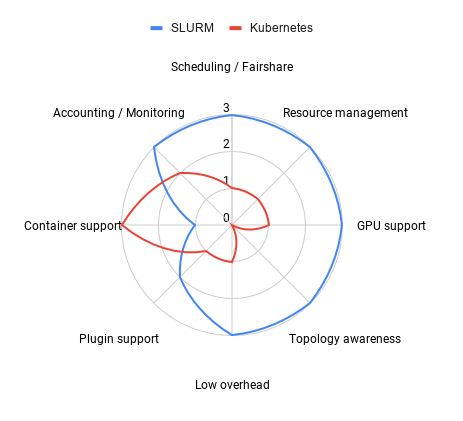
\includegraphics[width=\textwidth/2]{images/kube_vs_slurm.png}
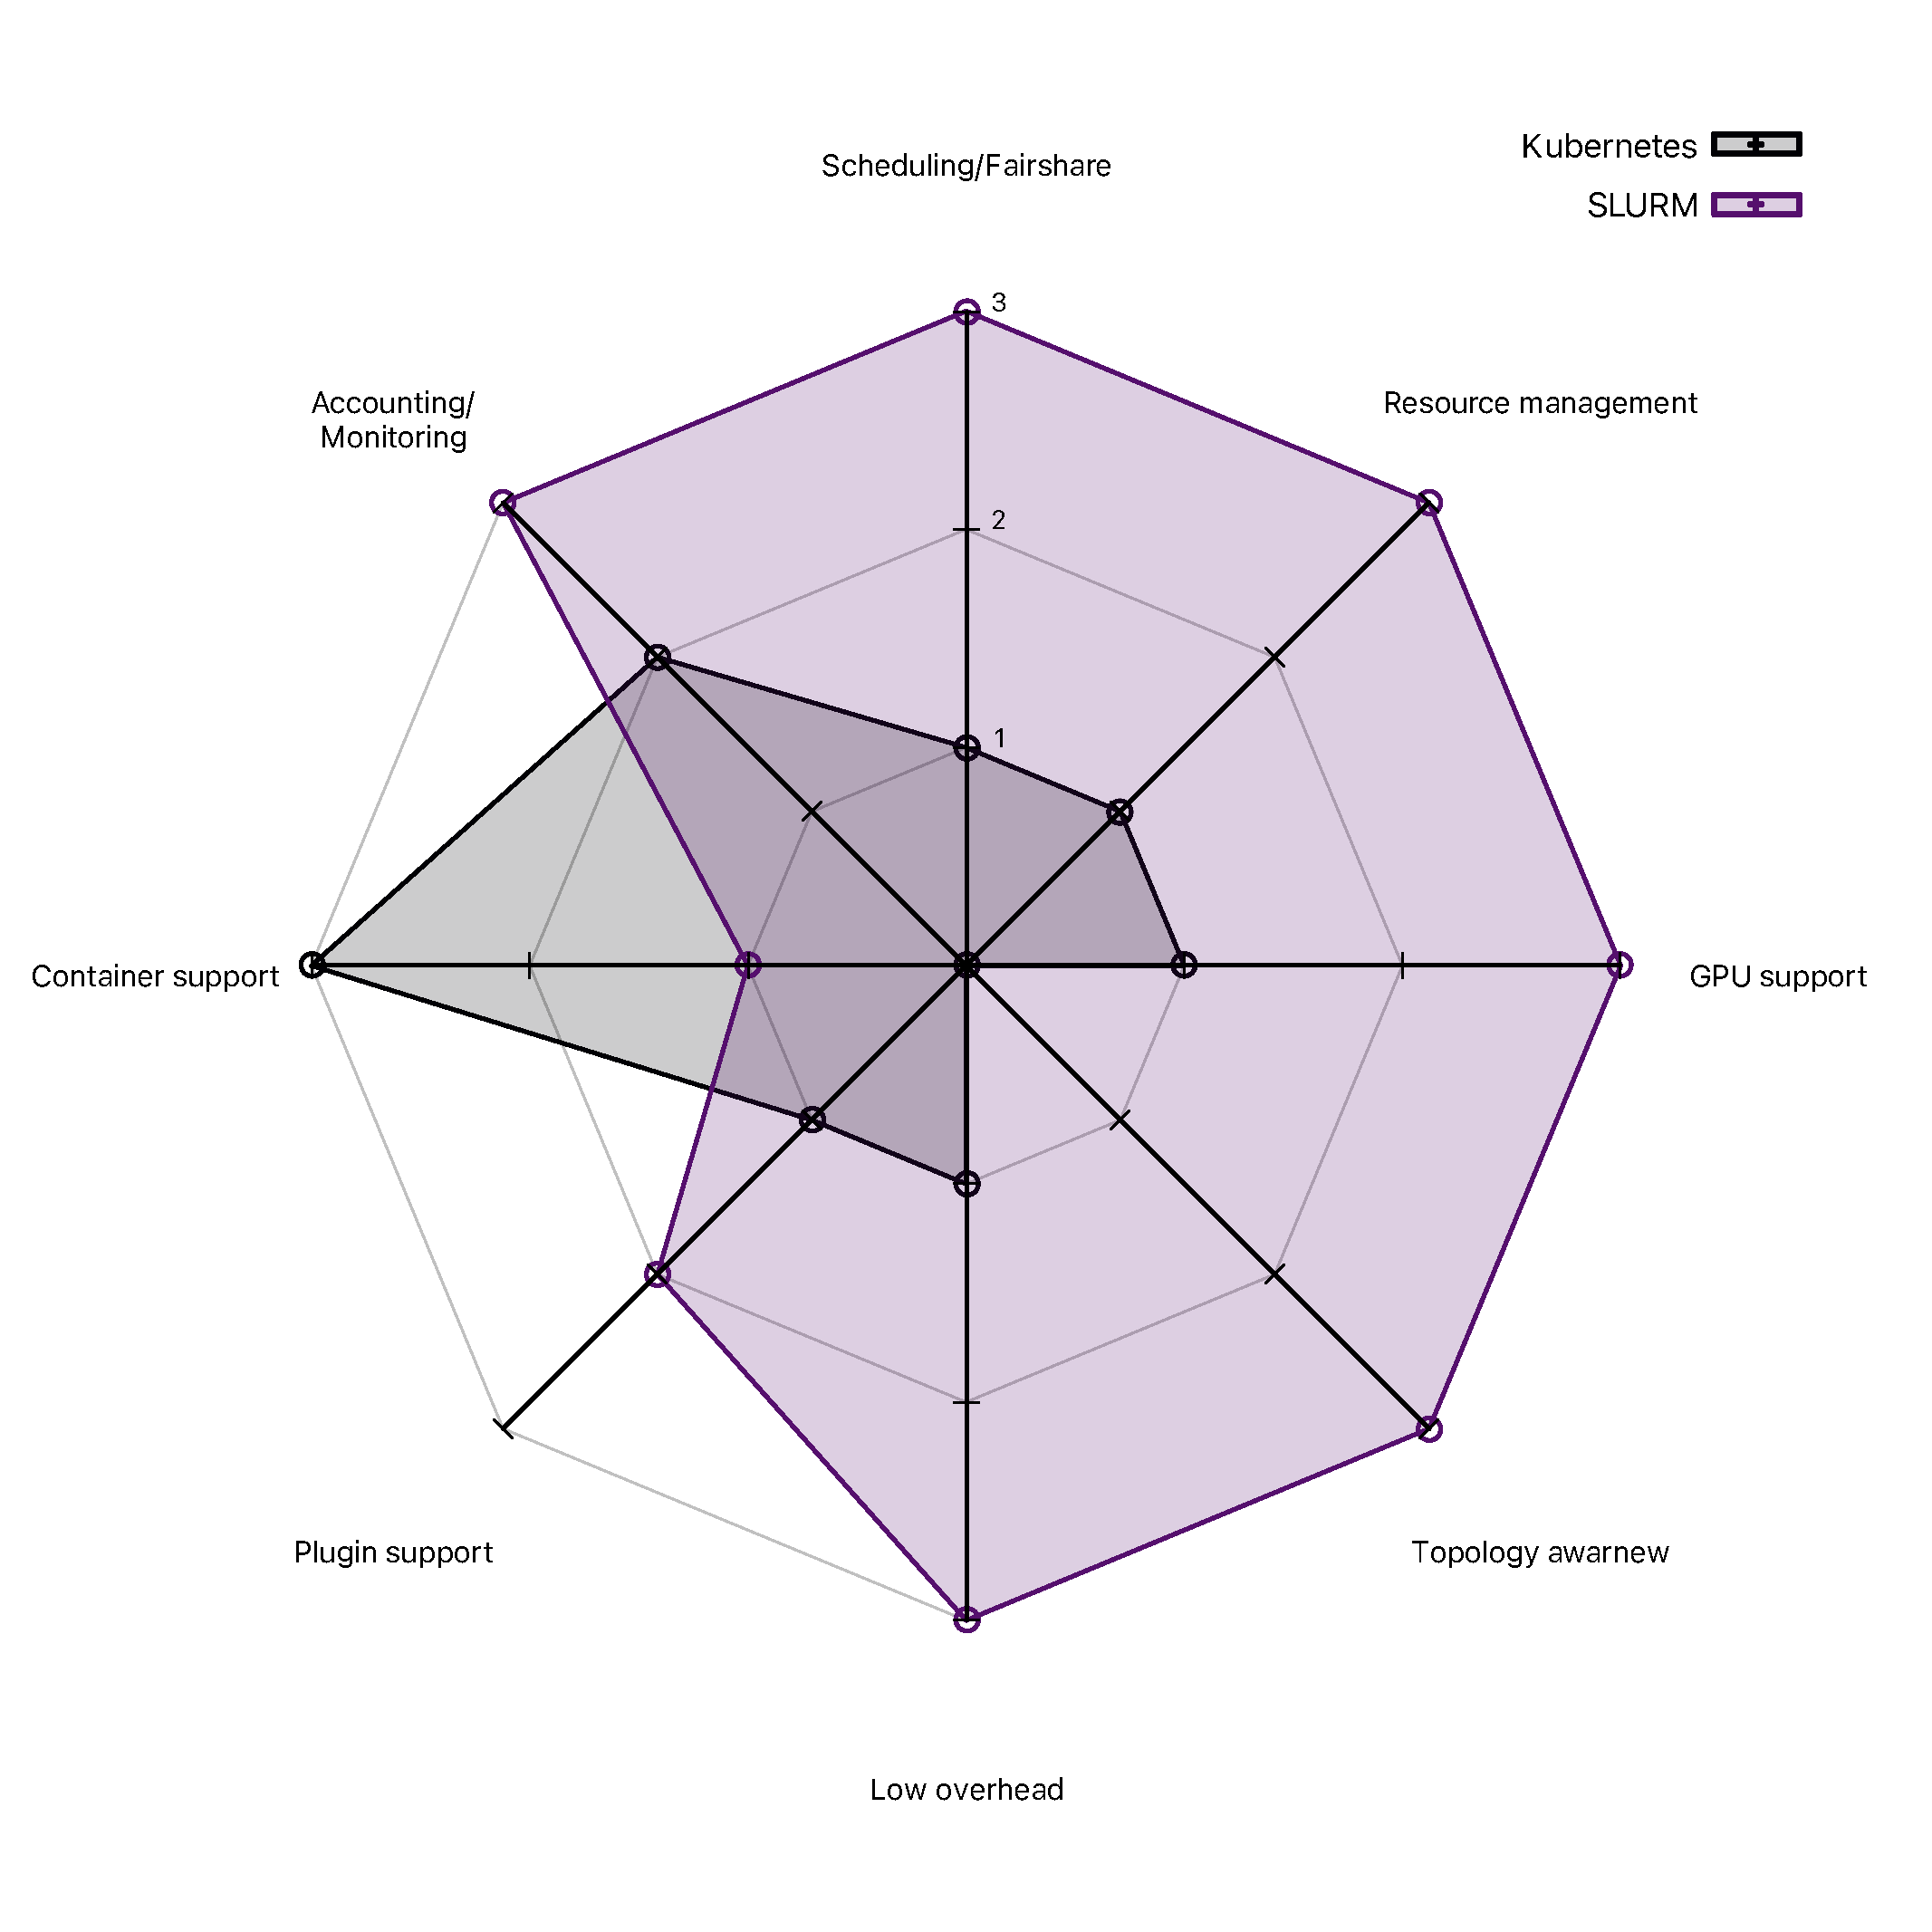
\includegraphics[scale=0.35]{images/kuber.pdf}
\caption{Strengths and weaknesses of SLURM and Kubernetes.}
\label{fig:kube_vs_slurm}
\end{figure}


\section{Conclusion}
In this research report we evaluated container technologies and orchestrators in the context of \gls{hpc}. Container usage in \gls{hpc} has some unique requirements. Such as interconnect and GPU support, an unprivileged runtime for security, and for collaborating within the \gls{hpc} community, an OCI standardized format. Furthermore, the preservation of cgroups (as is used in \gls{slurm}), ease of use with \gls{mpi} workloads and the ability to modify containers for customization. The latter requires a setup like e.g. the fakeroot option in Singularity, or by using Buildah which allows unprivileged container builds.

From the container technologies we tested and evaluated, none really disappointed. In terms of performance there was no clear winner. All container technologies performed equally to bare metal performance. However, Singularity and enroot have the best overall \gls{hpc} support (Figure \ref{fig:container_tech}). Where enroot especially excels for (nVidia) GPU workloads. Charliecloud looks very promising as well.

Traditional \gls{hpc} and Kubernetes co-existence is possible. However, there should be a valid use case for such a more complex and expensive setup \cite{cloudy-hutch}. While Kubernetes excels at orchestrating containers, containerized \gls{hpc} applications can be tricky to deploy on Kubernetes \cite{kubenetes-blog-meets-hpc}. Kubernetes is not designed for \gls{hpc}, hence it will never be as optimized as \gls{slurm}. However, in the effort to enable support of Big Data and Artificial Intelligence, Kubernetes is being enhanced with functionalities that will eventually interest the \gls{hpc} community. Furthermore, the trend of convergence between \gls{hpc} and Big Data may further motivate the usage of Kubernetes in \gls{hpc} in the future.


\newacronym{slurm}{SLURM}{Simple Linux Utility for Resource Management}
\newacronym{cca}{CCA}{Central Converged Architecture}
\newacronym{hpc}{HPC}{High Performance Computing}
\newacronym{mpi}{MPI}{Message Passing Interface}
\newacronym{cola}{COLA}{Customer Organisation LDAP Accounting Service}
\newacronym{rdma}{RDMA}{Remote Direct Memory Access}
\newacronym{rhel}{RHEL}{Red Hat Enterprise Linux}
\newacronym{oci}{OCI}{Open Containers Initiative}
\newacronym{nersc}{NERSC}{National Energy Research Scientific Computing Center}
\newacronym{sif}{SIF}{Singularity Image Format}
\newacronym{slug}{SLUG}{SLURM User Group}

\bibliographystyle{./bibliography/IEEEtran}
\bibliography{./bibliography/IEEEabrv,./bibliography/IEEEexample}

\end{document}